\documentclass[a4paper]{book}
\usepackage{a4wide}
\usepackage{makeidx}
\usepackage{graphicx}
\usepackage{multicol}
\usepackage{float}
\usepackage{listings}
\usepackage{color}
\usepackage{textcomp}
\usepackage{alltt}
\usepackage{times}
\usepackage{ifpdf}
\ifpdf
\usepackage[pdftex,
            pagebackref=true,
            colorlinks=true,
            linkcolor=blue,
            unicode
           ]{hyperref}
\else
\usepackage[ps2pdf,
            pagebackref=true,
            colorlinks=true,
            linkcolor=blue,
            unicode
           ]{hyperref}
\usepackage{pspicture}
\fi
\usepackage[utf8]{inputenc}
\usepackage{doxygen}
\lstset{language=C++,inputencoding=utf8,basicstyle=\footnotesize,breaklines=true,breakatwhitespace=true,tabsize=8,numbers=left }
\makeindex
\setcounter{tocdepth}{3}
\renewcommand{\footrulewidth}{0.4pt}
\begin{document}
\hypersetup{pageanchor=false}
\begin{titlepage}
\vspace*{7cm}
\begin{center}
{\Large Reference Manual}\\
\vspace*{1cm}
{\large Generated by Doxygen 1.6.3}\\
\vspace*{0.5cm}
{\small Mon Jun 18 04:18:14 2012}\\
\end{center}
\end{titlepage}
\clearemptydoublepage
\pagenumbering{roman}
\tableofcontents
\clearemptydoublepage
\pagenumbering{arabic}
\hypersetup{pageanchor=true}
\chapter{Class Index}
\section{Class Hierarchy}
This inheritance list is sorted roughly, but not completely, alphabetically:\begin{DoxyCompactList}
\item \contentsline{section}{CalculException}{\pageref{classCalculException}}{}
\item \contentsline{section}{Collection\_\-Onglet}{\pageref{classCollection__Onglet}}{}
\item \contentsline{section}{Collection\_\-onglet}{\pageref{classCollection__onglet}}{}
\item \contentsline{section}{Nombre::Data}{\pageref{classNombre_1_1Data}}{}
\begin{DoxyCompactList}
\item \contentsline{section}{Nombre::Complexe}{\pageref{classNombre_1_1Complexe}}{}
\item \contentsline{section}{Nombre::DataReelle}{\pageref{classNombre_1_1DataReelle}}{}
\begin{DoxyCompactList}
\item \contentsline{section}{Nombre::Entier}{\pageref{classNombre_1_1Entier}}{}
\item \contentsline{section}{Nombre::Rationnel}{\pageref{classNombre_1_1Rationnel}}{}
\item \contentsline{section}{Nombre::Reel}{\pageref{classNombre_1_1Reel}}{}
\end{DoxyCompactList}
\item \contentsline{section}{Nombre::Expression}{\pageref{classNombre_1_1Expression}}{}
\item \contentsline{section}{Nombre::Operateur}{\pageref{classNombre_1_1Operateur}}{}
\end{DoxyCompactList}
\item \contentsline{section}{DataGestion}{\pageref{classDataGestion}}{}
\item \contentsline{section}{Factory}{\pageref{classFactory}}{}
\begin{DoxyCompactList}
\item \contentsline{section}{ComplexeFactory}{\pageref{classComplexeFactory}}{}
\item \contentsline{section}{EntierFactory}{\pageref{classEntierFactory}}{}
\item \contentsline{section}{ExpressionFactory}{\pageref{classExpressionFactory}}{}
\item \contentsline{section}{OperateurFactory}{\pageref{classOperateurFactory}}{}
\item \contentsline{section}{RationnelFactory}{\pageref{classRationnelFactory}}{}
\item \contentsline{section}{ReelFactory}{\pageref{classReelFactory}}{}
\end{DoxyCompactList}
\item \contentsline{section}{ln}{\pageref{classln}}{}
\item \contentsline{section}{MainWindow}{\pageref{classMainWindow}}{}
\item \contentsline{section}{Onglet}{\pageref{classOnglet}}{}
\item \contentsline{section}{Operation::OperateurStrategy}{\pageref{classOperation_1_1OperateurStrategy}}{}
\begin{DoxyCompactList}
\item \contentsline{section}{Operation::Cos}{\pageref{classOperation_1_1Cos}}{}
\item \contentsline{section}{Operation::Cosh}{\pageref{classOperation_1_1Cosh}}{}
\item \contentsline{section}{Operation::Cube}{\pageref{classOperation_1_1Cube}}{}
\item \contentsline{section}{Operation::Div}{\pageref{classOperation_1_1Div}}{}
\item \contentsline{section}{Operation::Fact}{\pageref{classOperation_1_1Fact}}{}
\item \contentsline{section}{Operation::Inv}{\pageref{classOperation_1_1Inv}}{}
\item \contentsline{section}{Operation::Ln}{\pageref{classOperation_1_1Ln}}{}
\item \contentsline{section}{Operation::Log}{\pageref{classOperation_1_1Log}}{}
\item \contentsline{section}{Operation::Mod}{\pageref{classOperation_1_1Mod}}{}
\item \contentsline{section}{Operation::Moins}{\pageref{classOperation_1_1Moins}}{}
\item \contentsline{section}{Operation::Mult}{\pageref{classOperation_1_1Mult}}{}
\item \contentsline{section}{Operation::Plus}{\pageref{classOperation_1_1Plus}}{}
\item \contentsline{section}{Operation::Pow}{\pageref{classOperation_1_1Pow}}{}
\item \contentsline{section}{Operation::Sign}{\pageref{classOperation_1_1Sign}}{}
\item \contentsline{section}{Operation::Sin}{\pageref{classOperation_1_1Sin}}{}
\item \contentsline{section}{Operation::Sinh}{\pageref{classOperation_1_1Sinh}}{}
\item \contentsline{section}{Operation::Sqr}{\pageref{classOperation_1_1Sqr}}{}
\item \contentsline{section}{Operation::Sqrt}{\pageref{classOperation_1_1Sqrt}}{}
\item \contentsline{section}{Operation::Tan}{\pageref{classOperation_1_1Tan}}{}
\item \contentsline{section}{Operation::Tanh}{\pageref{classOperation_1_1Tanh}}{}
\end{DoxyCompactList}
\item \contentsline{section}{QStack}{\pageref{classQStack}}{}
\begin{DoxyCompactList}
\item \contentsline{section}{Pile$<$ T $>$}{\pageref{classPile}}{}
\end{DoxyCompactList}
\end{DoxyCompactList}

\chapter{Class Index}
\section{Class List}
Here are the classes, structs, unions and interfaces with brief descriptions:\begin{DoxyCompactList}
\item\contentsline{section}{\hyperlink{classCalculException}{CalculException} (Classe gerant les exceptions du programme )}{\pageref{classCalculException}}{}
\item\contentsline{section}{\hyperlink{classCollection__Onglet}{Collection\_\-Onglet} }{\pageref{classCollection__Onglet}}{}
\item\contentsline{section}{\hyperlink{classCollection__onglet}{Collection\_\-onglet} (Classe gérant l'ensemble des onglets de l'application )}{\pageref{classCollection__onglet}}{}
\item\contentsline{section}{\hyperlink{classNombre_1_1Complexe}{Nombre::Complexe} (Classe représentant les nombres complexes )}{\pageref{classNombre_1_1Complexe}}{}
\item\contentsline{section}{\hyperlink{classComplexeFactory}{ComplexeFactory} (Classe gérant la création des Complexe )}{\pageref{classComplexeFactory}}{}
\item\contentsline{section}{\hyperlink{classOperation_1_1Cos}{Operation::Cos} (Classe permettant d'effectuer l'opération cos )}{\pageref{classOperation_1_1Cos}}{}
\item\contentsline{section}{\hyperlink{classOperation_1_1Cosh}{Operation::Cosh} (Classe permettant d'effectuer l'opération cosh )}{\pageref{classOperation_1_1Cosh}}{}
\item\contentsline{section}{\hyperlink{classOperation_1_1Cube}{Operation::Cube} (Classe permettant d'effectuer l'opération cube )}{\pageref{classOperation_1_1Cube}}{}
\item\contentsline{section}{\hyperlink{classNombre_1_1Data}{Nombre::Data} (Classe dont hérite toutes les autres )}{\pageref{classNombre_1_1Data}}{}
\item\contentsline{section}{\hyperlink{classDataGestion}{DataGestion} (Classe servant de facade entre les donn�es du programme et l'interface Permet de g�rer tout le programme )}{\pageref{classDataGestion}}{}
\item\contentsline{section}{\hyperlink{classNombre_1_1DataReelle}{Nombre::DataReelle} (Classe mère de \hyperlink{classNombre_1_1Entier}{Entier}, \hyperlink{classNombre_1_1Rationnel}{Rationnel} et \hyperlink{classNombre_1_1Reel}{Reel} )}{\pageref{classNombre_1_1DataReelle}}{}
\item\contentsline{section}{\hyperlink{classOperation_1_1Div}{Operation::Div} (Classe permettant d'effectuer l'opération div )}{\pageref{classOperation_1_1Div}}{}
\item\contentsline{section}{\hyperlink{classNombre_1_1Entier}{Nombre::Entier} (Classe représentant les nombres entiers )}{\pageref{classNombre_1_1Entier}}{}
\item\contentsline{section}{\hyperlink{classEntierFactory}{EntierFactory} (Classe gérant la création des Entier )}{\pageref{classEntierFactory}}{}
\item\contentsline{section}{\hyperlink{classNombre_1_1Expression}{Nombre::Expression} (Classe représentant les expressions )}{\pageref{classNombre_1_1Expression}}{}
\item\contentsline{section}{\hyperlink{classExpressionFactory}{ExpressionFactory} (Classe gérant la création des Expression )}{\pageref{classExpressionFactory}}{}
\item\contentsline{section}{\hyperlink{classOperation_1_1Fact}{Operation::Fact} (Classe permettant d'effectuer l'opération factorielle )}{\pageref{classOperation_1_1Fact}}{}
\item\contentsline{section}{\hyperlink{classFactory}{Factory} (Classe gérant la création des différents éléments de données du programme )}{\pageref{classFactory}}{}
\item\contentsline{section}{\hyperlink{classOperation_1_1Inv}{Operation::Inv} (Classe permettant d'effectuer l'opération d'inversion )}{\pageref{classOperation_1_1Inv}}{}
\item\contentsline{section}{\hyperlink{classOperation_1_1Ln}{Operation::Ln} }{\pageref{classOperation_1_1Ln}}{}
\item\contentsline{section}{\hyperlink{classln}{ln} (Classe permettant d'effectuer l'opération ln )}{\pageref{classln}}{}
\item\contentsline{section}{\hyperlink{classOperation_1_1Log}{Operation::Log} (Classe permettant d'effectuer l'opération log10 )}{\pageref{classOperation_1_1Log}}{}
\item\contentsline{section}{\hyperlink{classMainWindow}{MainWindow} (Classe servant à coder l'interface )}{\pageref{classMainWindow}}{}
\item\contentsline{section}{\hyperlink{classOperation_1_1Mod}{Operation::Mod} (Classe permettant d'effectuer l'opération modulo )}{\pageref{classOperation_1_1Mod}}{}
\item\contentsline{section}{\hyperlink{classOperation_1_1Moins}{Operation::Moins} (Classe permettant d'effectuer l'opération moins )}{\pageref{classOperation_1_1Moins}}{}
\item\contentsline{section}{\hyperlink{classOperation_1_1Mult}{Operation::Mult} (Classe permettant d'effectuer l'opération multiplier )}{\pageref{classOperation_1_1Mult}}{}
\item\contentsline{section}{\hyperlink{classOnglet}{Onglet} (Classe représentant un onglet de la calculatrice )}{\pageref{classOnglet}}{}
\item\contentsline{section}{\hyperlink{classNombre_1_1Operateur}{Nombre::Operateur} (Classe représentant les opérateurs )}{\pageref{classNombre_1_1Operateur}}{}
\item\contentsline{section}{\hyperlink{classOperateurFactory}{OperateurFactory} (Classe gérant la création des Operateur )}{\pageref{classOperateurFactory}}{}
\item\contentsline{section}{\hyperlink{classOperation_1_1OperateurStrategy}{Operation::OperateurStrategy} (Classe virtuelle dont hérite toutes les stratégies )}{\pageref{classOperation_1_1OperateurStrategy}}{}
\item\contentsline{section}{\hyperlink{classPile}{Pile$<$ T $>$} (Classe pile, gardant les données du programme )}{\pageref{classPile}}{}
\item\contentsline{section}{\hyperlink{classOperation_1_1Plus}{Operation::Plus} (Classe permettant d'effectuer l'opération plus )}{\pageref{classOperation_1_1Plus}}{}
\item\contentsline{section}{\hyperlink{classOperation_1_1Pow}{Operation::Pow} (Classe permettant d'effectuer l'opération pow )}{\pageref{classOperation_1_1Pow}}{}
\item\contentsline{section}{\hyperlink{classQStack}{QStack} }{\pageref{classQStack}}{}
\item\contentsline{section}{\hyperlink{classNombre_1_1Rationnel}{Nombre::Rationnel} (Classe représentant les nombres rationnels )}{\pageref{classNombre_1_1Rationnel}}{}
\item\contentsline{section}{\hyperlink{classRationnelFactory}{RationnelFactory} (Classe gérant la création des Rationnel )}{\pageref{classRationnelFactory}}{}
\item\contentsline{section}{\hyperlink{classNombre_1_1Reel}{Nombre::Reel} (Classe représentant les nombres réels )}{\pageref{classNombre_1_1Reel}}{}
\item\contentsline{section}{\hyperlink{classReelFactory}{ReelFactory} (Classe gérant la création des Reel )}{\pageref{classReelFactory}}{}
\item\contentsline{section}{\hyperlink{classOperation_1_1Sign}{Operation::Sign} (Classe permettant d'effectuer l'opération sign )}{\pageref{classOperation_1_1Sign}}{}
\item\contentsline{section}{\hyperlink{classOperation_1_1Sin}{Operation::Sin} (Classe permettant d'effectuer l'opération sin )}{\pageref{classOperation_1_1Sin}}{}
\item\contentsline{section}{\hyperlink{classOperation_1_1Sinh}{Operation::Sinh} (Classe permettant d'effectuer l'opération sinh )}{\pageref{classOperation_1_1Sinh}}{}
\item\contentsline{section}{\hyperlink{classOperation_1_1Sqr}{Operation::Sqr} (Classe permettant d'effectuer l'opération carrée )}{\pageref{classOperation_1_1Sqr}}{}
\item\contentsline{section}{\hyperlink{classOperation_1_1Sqrt}{Operation::Sqrt} (Classe permettant d'effectuer l'opération racine carrée )}{\pageref{classOperation_1_1Sqrt}}{}
\item\contentsline{section}{\hyperlink{classOperation_1_1Tan}{Operation::Tan} (Classe permettant d'effectuer l'opération tan )}{\pageref{classOperation_1_1Tan}}{}
\item\contentsline{section}{\hyperlink{classOperation_1_1Tanh}{Operation::Tanh} (Classe permettant d'effectuer l'opération tanh )}{\pageref{classOperation_1_1Tanh}}{}
\end{DoxyCompactList}

\chapter{Class Documentation}
\hypertarget{classCalculException}{
\section{CalculException Class Reference}
\label{classCalculException}\index{CalculException@{CalculException}}
}


classe gerant les exceptions du programme  




{\ttfamily \#include $<$calculexception.h$>$}

\subsection*{Public Member Functions}
\begin{DoxyCompactItemize}
\item 
\hyperlink{classCalculException_a1b2321ee5a5aee7a5a939d19de8bb41c}{CalculException} (const std::string s)
\begin{DoxyCompactList}\small\item\em Constructeur. \item\end{DoxyCompactList}\item 
\hypertarget{classCalculException_a3c5a102baabcff71c5e988c9450022ae}{
const std::string \hyperlink{classCalculException_a3c5a102baabcff71c5e988c9450022ae}{getErreur} () const }
\label{classCalculException_a3c5a102baabcff71c5e988c9450022ae}

\begin{DoxyCompactList}\small\item\em retourne l'erreur \item\end{DoxyCompactList}\end{DoxyCompactItemize}


\subsection{Detailed Description}
classe gerant les exceptions du programme 

\subsection{Constructor \& Destructor Documentation}
\hypertarget{classCalculException_a1b2321ee5a5aee7a5a939d19de8bb41c}{
\index{CalculException@{CalculException}!CalculException@{CalculException}}
\index{CalculException@{CalculException}!CalculException@{CalculException}}
\subsubsection[{CalculException}]{\setlength{\rightskip}{0pt plus 5cm}CalculException::CalculException (const std::string {\em s})\hspace{0.3cm}{\ttfamily  \mbox{[}inline\mbox{]}}}}
\label{classCalculException_a1b2321ee5a5aee7a5a939d19de8bb41c}


Constructeur. 

Constructeur de la classe \hyperlink{classCalculException}{CalculException}


\begin{DoxyParams}{Parameters}
\item[{\em s}]: description de l'erreur \end{DoxyParams}


The documentation for this class was generated from the following file:\begin{DoxyCompactItemize}
\item 
calculexception.h\end{DoxyCompactItemize}

\hypertarget{classCollection__Onglet}{
\section{Collection\_\-Onglet Class Reference}
\label{classCollection__Onglet}\index{Collection\_\-Onglet@{Collection\_\-Onglet}}
}
\subsection*{Public Member Functions}
\begin{DoxyCompactItemize}
\item 
void \hyperlink{classCollection__Onglet_a56c620f3b31a3d6a0b3b20a9fa456739}{SetActif} (const int x)
\begin{DoxyCompactList}\small\item\em change l'entier actif de la classe \item\end{DoxyCompactList}\item 
\hypertarget{classCollection__Onglet_af6ee9683baa41fb0f06dd08fa0f379b6}{
int \hyperlink{classCollection__Onglet_af6ee9683baa41fb0f06dd08fa0f379b6}{GetActif} () const }
\label{classCollection__Onglet_af6ee9683baa41fb0f06dd08fa0f379b6}

\begin{DoxyCompactList}\small\item\em retourne actif \item\end{DoxyCompactList}\item 
void \hyperlink{classCollection__Onglet_a5abc570f57bbc5786de4bd2db933b059}{ajouterOnglet} (\hyperlink{classOnglet}{Onglet} $\ast$monOnglet)
\begin{DoxyCompactList}\small\item\em ajoute un onglet à la classe \item\end{DoxyCompactList}\item 
\hypertarget{classCollection__Onglet_a1a596730209916c34d6952f2bf2eaa62}{
int \hyperlink{classCollection__Onglet_a1a596730209916c34d6952f2bf2eaa62}{taille} ()}
\label{classCollection__Onglet_a1a596730209916c34d6952f2bf2eaa62}

\begin{DoxyCompactList}\small\item\em retourne la taille de la collection \item\end{DoxyCompactList}\item 
void \hyperlink{classCollection__Onglet_aa3cc4c74f4a47cd04f3dfa5d46c8a322}{supprimerOnglet} (int index)
\begin{DoxyCompactList}\small\item\em supprime un onglet de la collection \item\end{DoxyCompactList}\item 
\hypertarget{classCollection__Onglet_ac25f27894457f23d19b21c2c83f8c634}{
void \hyperlink{classCollection__Onglet_ac25f27894457f23d19b21c2c83f8c634}{saveContexte} ()}
\label{classCollection__Onglet_ac25f27894457f23d19b21c2c83f8c634}

\begin{DoxyCompactList}\small\item\em sauvegarde le contexte du programme dans un document xml \item\end{DoxyCompactList}\item 
\hypertarget{classCollection__Onglet_a7822474e999ad488e054d28f2a36be66}{
void \hyperlink{classCollection__Onglet_a7822474e999ad488e054d28f2a36be66}{chargerContexte} ()}
\label{classCollection__Onglet_a7822474e999ad488e054d28f2a36be66}

\begin{DoxyCompactList}\small\item\em charge le contexte du programme depuis un document xml \item\end{DoxyCompactList}\end{DoxyCompactItemize}
\subsection*{Static Public Member Functions}
\begin{DoxyCompactItemize}
\item 
\hypertarget{classCollection__Onglet_ae65253b1cf9c29937f2256db241732a8}{
static \hyperlink{classCollection__Onglet}{Collection\_\-Onglet} \& \hyperlink{classCollection__Onglet_ae65253b1cf9c29937f2256db241732a8}{GetInstance} ()}
\label{classCollection__Onglet_ae65253b1cf9c29937f2256db241732a8}

\begin{DoxyCompactList}\small\item\em retourne l'instance de la classe \item\end{DoxyCompactList}\item 
\hypertarget{classCollection__Onglet_ad18acceed361430b7def48e66f44b0b8}{
static void \hyperlink{classCollection__Onglet_ad18acceed361430b7def48e66f44b0b8}{ReleaseInstance} ()}
\label{classCollection__Onglet_ad18acceed361430b7def48e66f44b0b8}

\begin{DoxyCompactList}\small\item\em libère l'instance de la classe \item\end{DoxyCompactList}\end{DoxyCompactItemize}


\subsection{Member Function Documentation}
\hypertarget{classCollection__Onglet_a5abc570f57bbc5786de4bd2db933b059}{
\index{Collection\_\-Onglet@{Collection\_\-Onglet}!ajouterOnglet@{ajouterOnglet}}
\index{ajouterOnglet@{ajouterOnglet}!Collection_Onglet@{Collection\_\-Onglet}}
\subsubsection[{ajouterOnglet}]{\setlength{\rightskip}{0pt plus 5cm}void Collection\_\-Onglet::ajouterOnglet ({\bf Onglet} $\ast$ {\em monOnglet})}}
\label{classCollection__Onglet_a5abc570f57bbc5786de4bd2db933b059}


ajoute un onglet à la classe 


\begin{DoxyParams}{Parameters}
\item[{\em monOnglet}]: pointeur sur l'onglet à ajouter à la collection \end{DoxyParams}
\hypertarget{classCollection__Onglet_a56c620f3b31a3d6a0b3b20a9fa456739}{
\index{Collection\_\-Onglet@{Collection\_\-Onglet}!SetActif@{SetActif}}
\index{SetActif@{SetActif}!Collection_Onglet@{Collection\_\-Onglet}}
\subsubsection[{SetActif}]{\setlength{\rightskip}{0pt plus 5cm}void Collection\_\-Onglet::SetActif (const int {\em x})\hspace{0.3cm}{\ttfamily  \mbox{[}inline\mbox{]}}}}
\label{classCollection__Onglet_a56c620f3b31a3d6a0b3b20a9fa456739}


change l'entier actif de la classe 


\begin{DoxyParams}{Parameters}
\item[{\em x}]: nouvelle valeur de actif \end{DoxyParams}
\hypertarget{classCollection__Onglet_aa3cc4c74f4a47cd04f3dfa5d46c8a322}{
\index{Collection\_\-Onglet@{Collection\_\-Onglet}!supprimerOnglet@{supprimerOnglet}}
\index{supprimerOnglet@{supprimerOnglet}!Collection_Onglet@{Collection\_\-Onglet}}
\subsubsection[{supprimerOnglet}]{\setlength{\rightskip}{0pt plus 5cm}void Collection\_\-Onglet::supprimerOnglet (int {\em index})}}
\label{classCollection__Onglet_aa3cc4c74f4a47cd04f3dfa5d46c8a322}


supprime un onglet de la collection 


\begin{DoxyParams}{Parameters}
\item[{\em index}]: index de l'onglet à supprimer \end{DoxyParams}


The documentation for this class was generated from the following files:\begin{DoxyCompactItemize}
\item 
collection\_\-onglet.h\item 
collection\_\-onglet.cpp\end{DoxyCompactItemize}

\hypertarget{classCollection__onglet}{
\section{Collection\_\-onglet Class Reference}
\label{classCollection__onglet}\index{Collection\_\-onglet@{Collection\_\-onglet}}
}


classe gérant l'ensemble des onglets de l'application  




{\ttfamily \#include $<$collection\_\-onglet.h$>$}



\subsection{Detailed Description}
classe gérant l'ensemble des onglets de l'application 

The documentation for this class was generated from the following file:\begin{DoxyCompactItemize}
\item 
collection\_\-onglet.h\end{DoxyCompactItemize}

\hypertarget{classNombre_1_1Complexe}{
\section{Nombre::Complexe Class Reference}
\label{classNombre_1_1Complexe}\index{Nombre::Complexe@{Nombre::Complexe}}
}


classe représentant les nombres complexes  




{\ttfamily \#include $<$data.h$>$}

Inheritance diagram for Nombre::Complexe:\begin{figure}[H]
\begin{center}
\leavevmode
\includegraphics[height=2cm]{classNombre_1_1Complexe}
\end{center}
\end{figure}
\subsection*{Public Member Functions}
\begin{DoxyCompactItemize}
\item 
\hyperlink{classNombre_1_1Complexe_a752a5842b99a8e39bb89f4276d43e83c}{Complexe} (const \hyperlink{classNombre_1_1DataReelle}{DataReelle} \&r, const \hyperlink{classNombre_1_1DataReelle}{DataReelle} \&i)
\begin{DoxyCompactList}\small\item\em Constructeur. \item\end{DoxyCompactList}\item 
\hyperlink{classNombre_1_1Complexe_ac99372bf8b18c413b5c291b74eb846a4}{Complexe} (const QString \&s)
\begin{DoxyCompactList}\small\item\em Constructeur. \item\end{DoxyCompactList}\item 
\hyperlink{classNombre_1_1Complexe_abb864b5ffce7a6cc57c34ca06f331a60}{$\sim$Complexe} ()
\begin{DoxyCompactList}\small\item\em Destructeur. \item\end{DoxyCompactList}\item 
\hypertarget{classNombre_1_1Complexe_a7c8a9640dff617d6db1217604ebc6733}{
\hyperlink{classNombre_1_1DataReelle}{DataReelle} \& \hyperlink{classNombre_1_1Complexe_a7c8a9640dff617d6db1217604ebc6733}{getReel} () const }
\label{classNombre_1_1Complexe_a7c8a9640dff617d6db1217604ebc6733}

\begin{DoxyCompactList}\small\item\em retourne la partie réelle \item\end{DoxyCompactList}\item 
\hypertarget{classNombre_1_1Complexe_abda66d8237e6feb2f03178e59b6988a5}{
\hyperlink{classNombre_1_1DataReelle}{DataReelle} \& \hyperlink{classNombre_1_1Complexe_abda66d8237e6feb2f03178e59b6988a5}{getImaginaire} () const }
\label{classNombre_1_1Complexe_abda66d8237e6feb2f03178e59b6988a5}

\begin{DoxyCompactList}\small\item\em retourne la partie imaginaire \item\end{DoxyCompactList}\item 
void \hyperlink{classNombre_1_1Complexe_a498bde3887a4c785d51af6d64999f822}{setReel} (const \hyperlink{classNombre_1_1DataReelle}{DataReelle} \&r)
\begin{DoxyCompactList}\small\item\em change la partie réelle \item\end{DoxyCompactList}\item 
void \hyperlink{classNombre_1_1Complexe_af35fa6553144a161972f14d93c6ec954}{setImaginaire} (const \hyperlink{classNombre_1_1DataReelle}{DataReelle} \&i)
\begin{DoxyCompactList}\small\item\em change la partie imaginaire \item\end{DoxyCompactList}\item 
\hypertarget{classNombre_1_1Complexe_ab060a9a05c236ee293c85934702636cc}{
QString \& \hyperlink{classNombre_1_1Complexe_ab060a9a05c236ee293c85934702636cc}{toString} () const }
\label{classNombre_1_1Complexe_ab060a9a05c236ee293c85934702636cc}

\begin{DoxyCompactList}\small\item\em renvoie l'information en QString de la classe \item\end{DoxyCompactList}\item 
\hypertarget{classNombre_1_1Complexe_a40b54a55997c110e5e6b348374b33bf4}{
\hyperlink{classNombre_1_1Complexe}{Complexe} \& \hyperlink{classNombre_1_1Complexe_a40b54a55997c110e5e6b348374b33bf4}{clone} () const }
\label{classNombre_1_1Complexe_a40b54a55997c110e5e6b348374b33bf4}

\begin{DoxyCompactList}\small\item\em clone la classe \item\end{DoxyCompactList}\end{DoxyCompactItemize}
\subsection*{Static Public Member Functions}
\begin{DoxyCompactItemize}
\item 
static bool \hyperlink{classNombre_1_1Complexe_a6f932e9575a070a064868873d66962b8}{isComplexe} (const QString \&s)
\begin{DoxyCompactList}\small\item\em test si une string est un complexe \item\end{DoxyCompactList}\end{DoxyCompactItemize}


\subsection{Detailed Description}
classe représentant les nombres complexes 

\subsection{Constructor \& Destructor Documentation}
\hypertarget{classNombre_1_1Complexe_a752a5842b99a8e39bb89f4276d43e83c}{
\index{Nombre::Complexe@{Nombre::Complexe}!Complexe@{Complexe}}
\index{Complexe@{Complexe}!Nombre::Complexe@{Nombre::Complexe}}
\subsubsection[{Complexe}]{\setlength{\rightskip}{0pt plus 5cm}Nombre::Complexe::Complexe (const {\bf DataReelle} \& {\em r}, \/  const {\bf DataReelle} \& {\em i})\hspace{0.3cm}{\ttfamily  \mbox{[}inline\mbox{]}}}}
\label{classNombre_1_1Complexe_a752a5842b99a8e39bb89f4276d43e83c}


Constructeur. 

Constructeur de la classe


\begin{DoxyParams}{Parameters}
\item[{\em r}]: valeur de la partie réelle \item[{\em i}]: valeur de la partie imaginaire \end{DoxyParams}
\hypertarget{classNombre_1_1Complexe_ac99372bf8b18c413b5c291b74eb846a4}{
\index{Nombre::Complexe@{Nombre::Complexe}!Complexe@{Complexe}}
\index{Complexe@{Complexe}!Nombre::Complexe@{Nombre::Complexe}}
\subsubsection[{Complexe}]{\setlength{\rightskip}{0pt plus 5cm}Nombre::Complexe::Complexe (const QString \& {\em s})\hspace{0.3cm}{\ttfamily  \mbox{[}inline\mbox{]}}}}
\label{classNombre_1_1Complexe_ac99372bf8b18c413b5c291b74eb846a4}


Constructeur. 

Constructeur de la classe


\begin{DoxyParams}{Parameters}
\item[{\em s}]: qstring ayant la valeur du complexe \end{DoxyParams}
\hypertarget{classNombre_1_1Complexe_abb864b5ffce7a6cc57c34ca06f331a60}{
\index{Nombre::Complexe@{Nombre::Complexe}!$\sim$Complexe@{$\sim$Complexe}}
\index{$\sim$Complexe@{$\sim$Complexe}!Nombre::Complexe@{Nombre::Complexe}}
\subsubsection[{$\sim$Complexe}]{\setlength{\rightskip}{0pt plus 5cm}Nombre::Complexe::$\sim$Complexe ()\hspace{0.3cm}{\ttfamily  \mbox{[}inline\mbox{]}}}}
\label{classNombre_1_1Complexe_abb864b5ffce7a6cc57c34ca06f331a60}


Destructeur. 

Destructeur de la classe 

\subsection{Member Function Documentation}
\hypertarget{classNombre_1_1Complexe_a6f932e9575a070a064868873d66962b8}{
\index{Nombre::Complexe@{Nombre::Complexe}!isComplexe@{isComplexe}}
\index{isComplexe@{isComplexe}!Nombre::Complexe@{Nombre::Complexe}}
\subsubsection[{isComplexe}]{\setlength{\rightskip}{0pt plus 5cm}bool Nombre::Complexe::isComplexe (const QString \& {\em s})\hspace{0.3cm}{\ttfamily  \mbox{[}static\mbox{]}}}}
\label{classNombre_1_1Complexe_a6f932e9575a070a064868873d66962b8}


test si une string est un complexe 


\begin{DoxyParams}{Parameters}
\item[{\em s}]: la QString a tester \end{DoxyParams}
\hypertarget{classNombre_1_1Complexe_af35fa6553144a161972f14d93c6ec954}{
\index{Nombre::Complexe@{Nombre::Complexe}!setImaginaire@{setImaginaire}}
\index{setImaginaire@{setImaginaire}!Nombre::Complexe@{Nombre::Complexe}}
\subsubsection[{setImaginaire}]{\setlength{\rightskip}{0pt plus 5cm}void Nombre::Complexe::setImaginaire (const {\bf DataReelle} \& {\em i})\hspace{0.3cm}{\ttfamily  \mbox{[}inline\mbox{]}}}}
\label{classNombre_1_1Complexe_af35fa6553144a161972f14d93c6ec954}


change la partie imaginaire 


\begin{DoxyParams}{Parameters}
\item[{\em i}]: nouvelle valeur \end{DoxyParams}
\hypertarget{classNombre_1_1Complexe_a498bde3887a4c785d51af6d64999f822}{
\index{Nombre::Complexe@{Nombre::Complexe}!setReel@{setReel}}
\index{setReel@{setReel}!Nombre::Complexe@{Nombre::Complexe}}
\subsubsection[{setReel}]{\setlength{\rightskip}{0pt plus 5cm}void Nombre::Complexe::setReel (const {\bf DataReelle} \& {\em r})\hspace{0.3cm}{\ttfamily  \mbox{[}inline\mbox{]}}}}
\label{classNombre_1_1Complexe_a498bde3887a4c785d51af6d64999f822}


change la partie réelle 


\begin{DoxyParams}{Parameters}
\item[{\em i}]: nouvelle valeur \end{DoxyParams}


The documentation for this class was generated from the following files:\begin{DoxyCompactItemize}
\item 
data.h\item 
data.cpp\end{DoxyCompactItemize}

\hypertarget{classComplexeFactory}{
\section{ComplexeFactory Class Reference}
\label{classComplexeFactory}\index{ComplexeFactory@{ComplexeFactory}}
}


classe gérant la création des Complexe  




{\ttfamily \#include $<$factory.h$>$}

Inheritance diagram for ComplexeFactory:\begin{figure}[H]
\begin{center}
\leavevmode
\includegraphics[height=2cm]{classComplexeFactory}
\end{center}
\end{figure}
\subsection*{Static Public Member Functions}
\begin{DoxyCompactItemize}
\item 
static \hyperlink{classNombre_1_1Complexe}{Nombre::Complexe} \& \hyperlink{classComplexeFactory_a751c417a005259673accfc2a60fd62fd}{creer} (QString s)
\begin{DoxyCompactList}\small\item\em cree une nouvelle Data à partir d'une QString et la renvoie \item\end{DoxyCompactList}\end{DoxyCompactItemize}


\subsection{Detailed Description}
classe gérant la création des Complexe 

\subsection{Member Function Documentation}
\hypertarget{classComplexeFactory_a751c417a005259673accfc2a60fd62fd}{
\index{ComplexeFactory@{ComplexeFactory}!creer@{creer}}
\index{creer@{creer}!ComplexeFactory@{ComplexeFactory}}
\subsubsection[{creer}]{\setlength{\rightskip}{0pt plus 5cm}{\bf Complexe} \& ComplexeFactory::creer (QString {\em s})\hspace{0.3cm}{\ttfamily  \mbox{[}static\mbox{]}}}}
\label{classComplexeFactory_a751c417a005259673accfc2a60fd62fd}


cree une nouvelle Data à partir d'une QString et la renvoie 


\begin{DoxyParams}{Parameters}
\item[{\em s}]: QString servant de base à la création de la donnée \end{DoxyParams}


Reimplemented from \hyperlink{classFactory_afe37851e80172944b37491a952a28370}{Factory}.



The documentation for this class was generated from the following files:\begin{DoxyCompactItemize}
\item 
factory.h\item 
factory.cpp\end{DoxyCompactItemize}

\hypertarget{classOperation_1_1Cos}{
\section{Operation::Cos Class Reference}
\label{classOperation_1_1Cos}\index{Operation::Cos@{Operation::Cos}}
}


classe permettant d'effectuer l'opération cos  




{\ttfamily \#include $<$operateur.h$>$}

Inheritance diagram for Operation::Cos:\begin{figure}[H]
\begin{center}
\leavevmode
\includegraphics[height=2cm]{classOperation_1_1Cos}
\end{center}
\end{figure}
\subsection*{Public Member Functions}
\begin{DoxyCompactItemize}
\item 
\hyperlink{classNombre_1_1Data}{Data} \& \hyperlink{classOperation_1_1Cos_af1732358f2efad5b99a40732665b7bb7}{calcul} (\hyperlink{classPile}{Pile}$<$ \hyperlink{classNombre_1_1Data}{Data} $>$ $\ast$p)
\begin{DoxyCompactList}\small\item\em permet d'effectuer le calcul et de mettre la pile à jour \item\end{DoxyCompactList}\end{DoxyCompactItemize}


\subsection{Detailed Description}
classe permettant d'effectuer l'opération cos 

\subsection{Member Function Documentation}
\hypertarget{classOperation_1_1Cos_af1732358f2efad5b99a40732665b7bb7}{
\index{Operation::Cos@{Operation::Cos}!calcul@{calcul}}
\index{calcul@{calcul}!Operation::Cos@{Operation::Cos}}
\subsubsection[{calcul}]{\setlength{\rightskip}{0pt plus 5cm}{\bf Data}\& Operation::Cos::calcul ({\bf Pile}$<$ {\bf Data} $>$ $\ast$ {\em p})}}
\label{classOperation_1_1Cos_af1732358f2efad5b99a40732665b7bb7}


permet d'effectuer le calcul et de mettre la pile à jour 


\begin{DoxyParams}{Parameters}
\item[{\em p}]: la pile à mettre à jour après calcul \end{DoxyParams}


The documentation for this class was generated from the following file:\begin{DoxyCompactItemize}
\item 
operateur.h\end{DoxyCompactItemize}

\hypertarget{classOperation_1_1Cosh}{
\section{Operation::Cosh Class Reference}
\label{classOperation_1_1Cosh}\index{Operation::Cosh@{Operation::Cosh}}
}


classe permettant d'effectuer l'opération cosh  




{\ttfamily \#include $<$operateur.h$>$}

Inheritance diagram for Operation::Cosh:\begin{figure}[H]
\begin{center}
\leavevmode
\includegraphics[height=2cm]{classOperation_1_1Cosh}
\end{center}
\end{figure}
\subsection*{Public Member Functions}
\begin{DoxyCompactItemize}
\item 
\hyperlink{classNombre_1_1Data}{Data} \& \hyperlink{classOperation_1_1Cosh_a36990c65bccdadf30a8e3b967feb8d3a}{calcul} (\hyperlink{classPile}{Pile}$<$ \hyperlink{classNombre_1_1Data}{Data} $>$ $\ast$p)
\begin{DoxyCompactList}\small\item\em permet d'effectuer le calcul et de mettre la pile à jour \item\end{DoxyCompactList}\end{DoxyCompactItemize}


\subsection{Detailed Description}
classe permettant d'effectuer l'opération cosh 

\subsection{Member Function Documentation}
\hypertarget{classOperation_1_1Cosh_a36990c65bccdadf30a8e3b967feb8d3a}{
\index{Operation::Cosh@{Operation::Cosh}!calcul@{calcul}}
\index{calcul@{calcul}!Operation::Cosh@{Operation::Cosh}}
\subsubsection[{calcul}]{\setlength{\rightskip}{0pt plus 5cm}{\bf Data}\& Operation::Cosh::calcul ({\bf Pile}$<$ {\bf Data} $>$ $\ast$ {\em p})}}
\label{classOperation_1_1Cosh_a36990c65bccdadf30a8e3b967feb8d3a}


permet d'effectuer le calcul et de mettre la pile à jour 


\begin{DoxyParams}{Parameters}
\item[{\em p}]: la pile à mettre à jour après calcul \end{DoxyParams}


The documentation for this class was generated from the following file:\begin{DoxyCompactItemize}
\item 
operateur.h\end{DoxyCompactItemize}

\hypertarget{classOperation_1_1Cube}{
\section{Operation::Cube Class Reference}
\label{classOperation_1_1Cube}\index{Operation::Cube@{Operation::Cube}}
}


classe permettant d'effectuer l'opération cube  




{\ttfamily \#include $<$operateur.h$>$}

Inheritance diagram for Operation::Cube:\begin{figure}[H]
\begin{center}
\leavevmode
\includegraphics[height=2cm]{classOperation_1_1Cube}
\end{center}
\end{figure}
\subsection*{Public Member Functions}
\begin{DoxyCompactItemize}
\item 
\hyperlink{classNombre_1_1Data}{Data} \& \hyperlink{classOperation_1_1Cube_afe72197cd1178112ac3fcf6514c18042}{calcul} (\hyperlink{classPile}{Pile}$<$ \hyperlink{classNombre_1_1Data}{Data} $>$ $\ast$p)
\begin{DoxyCompactList}\small\item\em permet d'effectuer le calcul et de mettre la pile à jour \item\end{DoxyCompactList}\end{DoxyCompactItemize}


\subsection{Detailed Description}
classe permettant d'effectuer l'opération cube 

\subsection{Member Function Documentation}
\hypertarget{classOperation_1_1Cube_afe72197cd1178112ac3fcf6514c18042}{
\index{Operation::Cube@{Operation::Cube}!calcul@{calcul}}
\index{calcul@{calcul}!Operation::Cube@{Operation::Cube}}
\subsubsection[{calcul}]{\setlength{\rightskip}{0pt plus 5cm}{\bf Data}\& Operation::Cube::calcul ({\bf Pile}$<$ {\bf Data} $>$ $\ast$ {\em p})}}
\label{classOperation_1_1Cube_afe72197cd1178112ac3fcf6514c18042}


permet d'effectuer le calcul et de mettre la pile à jour 


\begin{DoxyParams}{Parameters}
\item[{\em p}]: la pile à mettre à jour après calcul \end{DoxyParams}


The documentation for this class was generated from the following file:\begin{DoxyCompactItemize}
\item 
operateur.h\end{DoxyCompactItemize}

\hypertarget{classNombre_1_1Data}{
\section{Nombre::Data Class Reference}
\label{classNombre_1_1Data}\index{Nombre::Data@{Nombre::Data}}
}


classe dont hérite toutes les autres  




{\ttfamily \#include $<$data.h$>$}

Inheritance diagram for Nombre::Data:\begin{figure}[H]
\begin{center}
\leavevmode
\includegraphics[height=3cm]{classNombre_1_1Data}
\end{center}
\end{figure}
\subsection*{Public Member Functions}
\begin{DoxyCompactItemize}
\item 
\hyperlink{classNombre_1_1Data_a5ecec0762dd46ac0feecc10d11d622bd}{Data} ()
\begin{DoxyCompactList}\small\item\em Constructeur. \item\end{DoxyCompactList}\item 
\hypertarget{classNombre_1_1Data_a5e1d3b57a2c241ececf01ba5e5c9cf6b}{
virtual QString \& \hyperlink{classNombre_1_1Data_a5e1d3b57a2c241ececf01ba5e5c9cf6b}{toString} () const =0}
\label{classNombre_1_1Data_a5e1d3b57a2c241ececf01ba5e5c9cf6b}

\begin{DoxyCompactList}\small\item\em renvoie l'information en QString de la classe \item\end{DoxyCompactList}\item 
\hypertarget{classNombre_1_1Data_a1f15fd4d8d98e6c8a87744247a019ad7}{
virtual \hyperlink{classNombre_1_1Data}{Data} \& \hyperlink{classNombre_1_1Data_a1f15fd4d8d98e6c8a87744247a019ad7}{clone} () const =0}
\label{classNombre_1_1Data_a1f15fd4d8d98e6c8a87744247a019ad7}

\begin{DoxyCompactList}\small\item\em clone la classe \item\end{DoxyCompactList}\end{DoxyCompactItemize}


\subsection{Detailed Description}
classe dont hérite toutes les autres 

\subsection{Constructor \& Destructor Documentation}
\hypertarget{classNombre_1_1Data_a5ecec0762dd46ac0feecc10d11d622bd}{
\index{Nombre::Data@{Nombre::Data}!Data@{Data}}
\index{Data@{Data}!Nombre::Data@{Nombre::Data}}
\subsubsection[{Data}]{\setlength{\rightskip}{0pt plus 5cm}Nombre::Data::Data ()\hspace{0.3cm}{\ttfamily  \mbox{[}inline\mbox{]}}}}
\label{classNombre_1_1Data_a5ecec0762dd46ac0feecc10d11d622bd}


Constructeur. 

Constructeur de la classe 

The documentation for this class was generated from the following file:\begin{DoxyCompactItemize}
\item 
data.h\end{DoxyCompactItemize}

\hypertarget{classDataGestion}{
\section{DataGestion Class Reference}
\label{classDataGestion}\index{DataGestion@{DataGestion}}
}


classe servant de facade entre les donn�es du programme et l'interface Permet de g�rer tout le programme  




{\ttfamily \#include $<$datagestion.h$>$}

\subsection*{Public Member Functions}
\begin{DoxyCompactItemize}
\item 
\hyperlink{classDataGestion_a5d90c5f766c07879a9e93a3e52e1a0c7}{DataGestion} ()
\begin{DoxyCompactList}\small\item\em Constructeur. \item\end{DoxyCompactList}\item 
\hyperlink{classDataGestion_a79229dcf9eb13b003468c8543a195311}{$\sim$DataGestion} ()
\begin{DoxyCompactList}\small\item\em Destructeur. \item\end{DoxyCompactList}\item 
\hypertarget{classDataGestion_a6bcdb2eab356aed159c8c2b9e315012f}{
\hyperlink{classPile}{Pile}$<$ \hyperlink{classNombre_1_1Data}{Data} $>$ \& \hyperlink{classDataGestion_a6bcdb2eab356aed159c8c2b9e315012f}{getStockage} () const }
\label{classDataGestion_a6bcdb2eab356aed159c8c2b9e315012f}

\begin{DoxyCompactList}\small\item\em retourne la pile de stockage \item\end{DoxyCompactList}\item 
\hypertarget{classDataGestion_afa53de93827d9a0902f60b803e3630dc}{
\hyperlink{classPile}{Pile}$<$ \hyperlink{classNombre_1_1Data}{Data} $>$ \& \hyperlink{classDataGestion_afa53de93827d9a0902f60b803e3630dc}{getRetablir} () const }
\label{classDataGestion_afa53de93827d9a0902f60b803e3630dc}

\begin{DoxyCompactList}\small\item\em retourne la pile r�tablir \item\end{DoxyCompactList}\item 
\hypertarget{classDataGestion_adf1fe14cc9df3df0c96fe316cb620090}{
\hyperlink{classPile}{Pile}$<$ QString $>$ \& \hyperlink{classDataGestion_adf1fe14cc9df3df0c96fe316cb620090}{getAffichage} () const }
\label{classDataGestion_adf1fe14cc9df3df0c96fe316cb620090}

\begin{DoxyCompactList}\small\item\em retourne la pile d'affichage \item\end{DoxyCompactList}\item 
void \hyperlink{classDataGestion_a4ceeb6d89c71d7b351580ddf09666d77}{setStockage} (\hyperlink{classPile}{Pile}$<$ \hyperlink{classNombre_1_1Data}{Data} $>$ \&p)
\begin{DoxyCompactList}\small\item\em change la pile de stockage \item\end{DoxyCompactList}\item 
void \hyperlink{classDataGestion_a8f277703ec10e113a9dc15770efa2172}{setRetablir} (\hyperlink{classPile}{Pile}$<$ \hyperlink{classNombre_1_1Data}{Data} $>$ \&p)
\begin{DoxyCompactList}\small\item\em change la pile r�tablir \item\end{DoxyCompactList}\item 
void \hyperlink{classDataGestion_a694f774208e240a7be99010b89f0d1db}{setAffichage} (\hyperlink{classPile}{Pile}$<$ QString $>$ \&p)
\begin{DoxyCompactList}\small\item\em change la pile d'affichage \item\end{DoxyCompactList}\item 
\hypertarget{classDataGestion_a3cc348effd70a7ca7f1bf1a5dfb826cc}{
\hyperlink{classFactory}{Factory} \& \hyperlink{classDataGestion_a3cc348effd70a7ca7f1bf1a5dfb826cc}{getFactory} () const }
\label{classDataGestion_a3cc348effd70a7ca7f1bf1a5dfb826cc}

\begin{DoxyCompactList}\small\item\em retourne l'instance de la factory \item\end{DoxyCompactList}\item 
void \hyperlink{classDataGestion_a549e4be0e31d71db589e8028ce2f9f09}{parse} (QString expression)
\begin{DoxyCompactList}\small\item\em d�code une entr�e utlisateur \item\end{DoxyCompactList}\item 
void \hyperlink{classDataGestion_a000582dcd78e4058a05efd3180f84a7c}{calcul} ()
\begin{DoxyCompactList}\small\item\em effectue le calcul \item\end{DoxyCompactList}\item 
\hypertarget{classDataGestion_ae6cfb21caca7d8def491a174490618b3}{
void \hyperlink{classDataGestion_ae6cfb21caca7d8def491a174490618b3}{annuler} ()}
\label{classDataGestion_ae6cfb21caca7d8def491a174490618b3}

\begin{DoxyCompactList}\small\item\em annule les x derni�res op�rations sur la pile de stockage \item\end{DoxyCompactList}\item 
\hypertarget{classDataGestion_a26812b599e4be247ba00747a78806331}{
void \hyperlink{classDataGestion_a26812b599e4be247ba00747a78806331}{retablir} ()}
\label{classDataGestion_a26812b599e4be247ba00747a78806331}

\begin{DoxyCompactList}\small\item\em r�tablit les x derni�res op�rations sur la pile de stockage \item\end{DoxyCompactList}\end{DoxyCompactItemize}


\subsection{Detailed Description}
classe servant de facade entre les donn�es du programme et l'interface Permet de g�rer tout le programme 

\subsection{Constructor \& Destructor Documentation}
\hypertarget{classDataGestion_a5d90c5f766c07879a9e93a3e52e1a0c7}{
\index{DataGestion@{DataGestion}!DataGestion@{DataGestion}}
\index{DataGestion@{DataGestion}!DataGestion@{DataGestion}}
\subsubsection[{DataGestion}]{\setlength{\rightskip}{0pt plus 5cm}DataGestion::DataGestion ()}}
\label{classDataGestion_a5d90c5f766c07879a9e93a3e52e1a0c7}


Constructeur. 

Constructeur de la classe \hypertarget{classDataGestion_a79229dcf9eb13b003468c8543a195311}{
\index{DataGestion@{DataGestion}!$\sim$DataGestion@{$\sim$DataGestion}}
\index{$\sim$DataGestion@{$\sim$DataGestion}!DataGestion@{DataGestion}}
\subsubsection[{$\sim$DataGestion}]{\setlength{\rightskip}{0pt plus 5cm}DataGestion::$\sim$DataGestion ()}}
\label{classDataGestion_a79229dcf9eb13b003468c8543a195311}


Destructeur. 

Destructeur de la classe 

\subsection{Member Function Documentation}
\hypertarget{classDataGestion_a000582dcd78e4058a05efd3180f84a7c}{
\index{DataGestion@{DataGestion}!calcul@{calcul}}
\index{calcul@{calcul}!DataGestion@{DataGestion}}
\subsubsection[{calcul}]{\setlength{\rightskip}{0pt plus 5cm}void DataGestion::calcul ()}}
\label{classDataGestion_a000582dcd78e4058a05efd3180f84a7c}


effectue le calcul 

Utilise le pattern strategy des op�rations pour calculer et mettre les piles � jour \hypertarget{classDataGestion_a549e4be0e31d71db589e8028ce2f9f09}{
\index{DataGestion@{DataGestion}!parse@{parse}}
\index{parse@{parse}!DataGestion@{DataGestion}}
\subsubsection[{parse}]{\setlength{\rightskip}{0pt plus 5cm}void DataGestion::parse (QString {\em expression})}}
\label{classDataGestion_a549e4be0e31d71db589e8028ce2f9f09}


d�code une entr�e utlisateur 

Appel la factory, cr�e les Data qu'il faut, remplit les piles et appelle calcul


\begin{DoxyParams}{Parameters}
\item[{\em expression}]: la QStrign entr�e par l'utilisateur \end{DoxyParams}
\hypertarget{classDataGestion_a694f774208e240a7be99010b89f0d1db}{
\index{DataGestion@{DataGestion}!setAffichage@{setAffichage}}
\index{setAffichage@{setAffichage}!DataGestion@{DataGestion}}
\subsubsection[{setAffichage}]{\setlength{\rightskip}{0pt plus 5cm}void DataGestion::setAffichage ({\bf Pile}$<$ QString $>$ \& {\em p})\hspace{0.3cm}{\ttfamily  \mbox{[}inline\mbox{]}}}}
\label{classDataGestion_a694f774208e240a7be99010b89f0d1db}


change la pile d'affichage 


\begin{DoxyParams}{Parameters}
\item[{\em p}]: nouvelle pile \end{DoxyParams}
\hypertarget{classDataGestion_a8f277703ec10e113a9dc15770efa2172}{
\index{DataGestion@{DataGestion}!setRetablir@{setRetablir}}
\index{setRetablir@{setRetablir}!DataGestion@{DataGestion}}
\subsubsection[{setRetablir}]{\setlength{\rightskip}{0pt plus 5cm}void DataGestion::setRetablir ({\bf Pile}$<$ {\bf Data} $>$ \& {\em p})\hspace{0.3cm}{\ttfamily  \mbox{[}inline\mbox{]}}}}
\label{classDataGestion_a8f277703ec10e113a9dc15770efa2172}


change la pile r�tablir 


\begin{DoxyParams}{Parameters}
\item[{\em p}]: nouvelle pile \end{DoxyParams}
\hypertarget{classDataGestion_a4ceeb6d89c71d7b351580ddf09666d77}{
\index{DataGestion@{DataGestion}!setStockage@{setStockage}}
\index{setStockage@{setStockage}!DataGestion@{DataGestion}}
\subsubsection[{setStockage}]{\setlength{\rightskip}{0pt plus 5cm}void DataGestion::setStockage ({\bf Pile}$<$ {\bf Data} $>$ \& {\em p})\hspace{0.3cm}{\ttfamily  \mbox{[}inline\mbox{]}}}}
\label{classDataGestion_a4ceeb6d89c71d7b351580ddf09666d77}


change la pile de stockage 


\begin{DoxyParams}{Parameters}
\item[{\em p}]: nouvelle pile \end{DoxyParams}


The documentation for this class was generated from the following files:\begin{DoxyCompactItemize}
\item 
datagestion.h\item 
datagestion.cpp\end{DoxyCompactItemize}

\hypertarget{classNombre_1_1DataReelle}{
\section{Nombre::DataReelle Class Reference}
\label{classNombre_1_1DataReelle}\index{Nombre::DataReelle@{Nombre::DataReelle}}
}


classe mère de \hyperlink{classNombre_1_1Entier}{Entier}, \hyperlink{classNombre_1_1Rationnel}{Rationnel} et \hyperlink{classNombre_1_1Reel}{Reel}  




{\ttfamily \#include $<$data.h$>$}

Inheritance diagram for Nombre::DataReelle:\begin{figure}[H]
\begin{center}
\leavevmode
\includegraphics[height=3cm]{classNombre_1_1DataReelle}
\end{center}
\end{figure}
\subsection*{Public Member Functions}
\begin{DoxyCompactItemize}
\item 
\hyperlink{classNombre_1_1DataReelle_a3360b818a88c03f35499c1cd8cdb614b}{DataReelle} ()
\begin{DoxyCompactList}\small\item\em Constructeur. \item\end{DoxyCompactList}\item 
\hypertarget{classNombre_1_1DataReelle_aa267b82217eae17427ef10be250dfac7}{
virtual \hyperlink{classNombre_1_1DataReelle}{DataReelle} \& \hyperlink{classNombre_1_1DataReelle_aa267b82217eae17427ef10be250dfac7}{clone} () const =0}
\label{classNombre_1_1DataReelle_aa267b82217eae17427ef10be250dfac7}

\begin{DoxyCompactList}\small\item\em clone la classe \item\end{DoxyCompactList}\item 
\hypertarget{classNombre_1_1DataReelle_aef66518fe7007b3673028ffce6d8f1c8}{
virtual \hyperlink{classNombre_1_1Entier}{Nombre::Entier} \& \hyperlink{classNombre_1_1DataReelle_aef66518fe7007b3673028ffce6d8f1c8}{toEntier} () const =0}
\label{classNombre_1_1DataReelle_aef66518fe7007b3673028ffce6d8f1c8}

\begin{DoxyCompactList}\small\item\em transforme la \hyperlink{classNombre_1_1Data}{Data} en \hyperlink{classNombre_1_1Entier}{Entier} \item\end{DoxyCompactList}\item 
\hypertarget{classNombre_1_1DataReelle_ae84e9c4bb3e792eab7ce487778089529}{
virtual \hyperlink{classNombre_1_1Reel}{Nombre::Reel} \& \hyperlink{classNombre_1_1DataReelle_ae84e9c4bb3e792eab7ce487778089529}{toReel} () const =0}
\label{classNombre_1_1DataReelle_ae84e9c4bb3e792eab7ce487778089529}

\begin{DoxyCompactList}\small\item\em transforme la \hyperlink{classNombre_1_1Data}{Data} en \hyperlink{classNombre_1_1Reel}{Reel} \item\end{DoxyCompactList}\item 
\hypertarget{classNombre_1_1DataReelle_af047f3ec5bf59e3183b185f96af134a4}{
virtual \hyperlink{classNombre_1_1Rationnel}{Nombre::Rationnel} \& \hyperlink{classNombre_1_1DataReelle_af047f3ec5bf59e3183b185f96af134a4}{toRationnel} () const =0}
\label{classNombre_1_1DataReelle_af047f3ec5bf59e3183b185f96af134a4}

\begin{DoxyCompactList}\small\item\em transforme la \hyperlink{classNombre_1_1Data}{Data} en \hyperlink{classNombre_1_1Rationnel}{Rationnel} \item\end{DoxyCompactList}\end{DoxyCompactItemize}


\subsection{Detailed Description}
classe mère de \hyperlink{classNombre_1_1Entier}{Entier}, \hyperlink{classNombre_1_1Rationnel}{Rationnel} et \hyperlink{classNombre_1_1Reel}{Reel} 

\subsection{Constructor \& Destructor Documentation}
\hypertarget{classNombre_1_1DataReelle_a3360b818a88c03f35499c1cd8cdb614b}{
\index{Nombre::DataReelle@{Nombre::DataReelle}!DataReelle@{DataReelle}}
\index{DataReelle@{DataReelle}!Nombre::DataReelle@{Nombre::DataReelle}}
\subsubsection[{DataReelle}]{\setlength{\rightskip}{0pt plus 5cm}Nombre::DataReelle::DataReelle ()\hspace{0.3cm}{\ttfamily  \mbox{[}inline\mbox{]}}}}
\label{classNombre_1_1DataReelle_a3360b818a88c03f35499c1cd8cdb614b}


Constructeur. 

Constructeur de la classe 

The documentation for this class was generated from the following file:\begin{DoxyCompactItemize}
\item 
data.h\end{DoxyCompactItemize}

\hypertarget{classOperation_1_1Div}{
\section{Operation::Div Class Reference}
\label{classOperation_1_1Div}\index{Operation::Div@{Operation::Div}}
}


classe permettant d'effectuer l'opération div  




{\ttfamily \#include $<$operateur.h$>$}

Inheritance diagram for Operation::Div:\begin{figure}[H]
\begin{center}
\leavevmode
\includegraphics[height=2cm]{classOperation_1_1Div}
\end{center}
\end{figure}
\subsection*{Public Member Functions}
\begin{DoxyCompactItemize}
\item 
\hyperlink{classNombre_1_1Complexe}{Complexe} \& \hyperlink{classOperation_1_1Div_a32cea3648beaa64f84b33545a0c328f8}{divComplexe} (const \hyperlink{classNombre_1_1Complexe}{Complexe} \&a, const \hyperlink{classNombre_1_1Complexe}{Complexe} \&b)
\begin{DoxyCompactList}\small\item\em permet d'effectuer l'opération div pour deux complexes \item\end{DoxyCompactList}\item 
\hyperlink{classNombre_1_1Rationnel}{Rationnel} \& \hyperlink{classOperation_1_1Div_afbe5105e27ceea4490a71155c7229541}{divRationnel} (const \hyperlink{classNombre_1_1Rationnel}{Rationnel} \&r1, const \hyperlink{classNombre_1_1Rationnel}{Rationnel} \&r2)
\begin{DoxyCompactList}\small\item\em permet d'effectuer l'opération div pour deux rationnels \item\end{DoxyCompactList}\item 
\hyperlink{classNombre_1_1Data}{Data} \& \hyperlink{classOperation_1_1Div_a4530654b1b81fdeadb4f1532fcaea85d}{calcul} (\hyperlink{classPile}{Pile}$<$ \hyperlink{classNombre_1_1Data}{Data} $>$ $\ast$p)
\begin{DoxyCompactList}\small\item\em permet d'effectuer le calcul et de mettre la pile à jour \item\end{DoxyCompactList}\end{DoxyCompactItemize}


\subsection{Detailed Description}
classe permettant d'effectuer l'opération div 

\subsection{Member Function Documentation}
\hypertarget{classOperation_1_1Div_a4530654b1b81fdeadb4f1532fcaea85d}{
\index{Operation::Div@{Operation::Div}!calcul@{calcul}}
\index{calcul@{calcul}!Operation::Div@{Operation::Div}}
\subsubsection[{calcul}]{\setlength{\rightskip}{0pt plus 5cm}{\bf Data}\& Operation::Div::calcul ({\bf Pile}$<$ {\bf Data} $>$ $\ast$ {\em p})}}
\label{classOperation_1_1Div_a4530654b1b81fdeadb4f1532fcaea85d}


permet d'effectuer le calcul et de mettre la pile à jour 


\begin{DoxyParams}{Parameters}
\item[{\em p}]: la pile à mettre à jour après calcul \end{DoxyParams}
\hypertarget{classOperation_1_1Div_a32cea3648beaa64f84b33545a0c328f8}{
\index{Operation::Div@{Operation::Div}!divComplexe@{divComplexe}}
\index{divComplexe@{divComplexe}!Operation::Div@{Operation::Div}}
\subsubsection[{divComplexe}]{\setlength{\rightskip}{0pt plus 5cm}{\bf Complexe}\& Operation::Div::divComplexe (const {\bf Complexe} \& {\em a}, \/  const {\bf Complexe} \& {\em b})}}
\label{classOperation_1_1Div_a32cea3648beaa64f84b33545a0c328f8}


permet d'effectuer l'opération div pour deux complexes 


\begin{DoxyParams}{Parameters}
\item[{\em a}]: le premier complexe \item[{\em b}]: le second complexe \end{DoxyParams}
\hypertarget{classOperation_1_1Div_afbe5105e27ceea4490a71155c7229541}{
\index{Operation::Div@{Operation::Div}!divRationnel@{divRationnel}}
\index{divRationnel@{divRationnel}!Operation::Div@{Operation::Div}}
\subsubsection[{divRationnel}]{\setlength{\rightskip}{0pt plus 5cm}{\bf Rationnel}\& Operation::Div::divRationnel (const {\bf Rationnel} \& {\em r1}, \/  const {\bf Rationnel} \& {\em r2})}}
\label{classOperation_1_1Div_afbe5105e27ceea4490a71155c7229541}


permet d'effectuer l'opération div pour deux rationnels 


\begin{DoxyParams}{Parameters}
\item[{\em r1}]: le premier rationnel \item[{\em r2}]: le second rationnel \end{DoxyParams}


The documentation for this class was generated from the following file:\begin{DoxyCompactItemize}
\item 
operateur.h\end{DoxyCompactItemize}

\hypertarget{classNombre_1_1Entier}{
\section{Nombre::Entier Class Reference}
\label{classNombre_1_1Entier}\index{Nombre::Entier@{Nombre::Entier}}
}


classe représentant les nombres entiers  




{\ttfamily \#include $<$data.h$>$}

Inheritance diagram for Nombre::Entier:\begin{figure}[H]
\begin{center}
\leavevmode
\includegraphics[height=3cm]{classNombre_1_1Entier}
\end{center}
\end{figure}
\subsection*{Public Member Functions}
\begin{DoxyCompactItemize}
\item 
\hyperlink{classNombre_1_1Entier_aba1baf196e52fb9ea0398e5c5695bf61}{Entier} (int i)
\begin{DoxyCompactList}\small\item\em Constructeur. \item\end{DoxyCompactList}\item 
\hyperlink{classNombre_1_1Entier_a15923a12f9ef441d981f7c8b0977d233}{Entier} (const \hyperlink{classNombre_1_1Entier}{Entier} \&e)
\begin{DoxyCompactList}\small\item\em Constructeur par recopie. \item\end{DoxyCompactList}\item 
\hyperlink{classNombre_1_1Entier_ae18e68f53e56a1ed8e951cb43b7b34d1}{Entier} (const QString \&s)
\begin{DoxyCompactList}\small\item\em Constructeur. \item\end{DoxyCompactList}\item 
\hypertarget{classNombre_1_1Entier_a77282a0f57f0bdaecb5abceab8ad38d1}{
int \hyperlink{classNombre_1_1Entier_a77282a0f57f0bdaecb5abceab8ad38d1}{getValeur} () const }
\label{classNombre_1_1Entier_a77282a0f57f0bdaecb5abceab8ad38d1}

\begin{DoxyCompactList}\small\item\em retourne la valeur \item\end{DoxyCompactList}\item 
void \hyperlink{classNombre_1_1Entier_a434f40deb776ef9f128629095d130bf2}{setValeur} (int i)
\begin{DoxyCompactList}\small\item\em donne une nouvelle valeur \item\end{DoxyCompactList}\item 
\hypertarget{classNombre_1_1Entier_ad2ad3a58c27c2a288f0879eac1f3d73d}{
\hyperlink{classNombre_1_1Entier}{Entier} \& \hyperlink{classNombre_1_1Entier_ad2ad3a58c27c2a288f0879eac1f3d73d}{toEntier} () const }
\label{classNombre_1_1Entier_ad2ad3a58c27c2a288f0879eac1f3d73d}

\begin{DoxyCompactList}\small\item\em transforme la \hyperlink{classNombre_1_1Data}{Data} en \hyperlink{classNombre_1_1Entier}{Entier} \item\end{DoxyCompactList}\item 
\hypertarget{classNombre_1_1Entier_a1844bb6f59d844abdd10c1b9d252ae49}{
\hyperlink{classNombre_1_1Reel}{Reel} \& \hyperlink{classNombre_1_1Entier_a1844bb6f59d844abdd10c1b9d252ae49}{toReel} () const }
\label{classNombre_1_1Entier_a1844bb6f59d844abdd10c1b9d252ae49}

\begin{DoxyCompactList}\small\item\em transforme la \hyperlink{classNombre_1_1Data}{Data} en \hyperlink{classNombre_1_1Reel}{Reel} \item\end{DoxyCompactList}\item 
\hypertarget{classNombre_1_1Entier_a74bc77a7d8ea295c30c4acebf8539d32}{
\hyperlink{classNombre_1_1Rationnel}{Rationnel} \& \hyperlink{classNombre_1_1Entier_a74bc77a7d8ea295c30c4acebf8539d32}{toRationnel} () const }
\label{classNombre_1_1Entier_a74bc77a7d8ea295c30c4acebf8539d32}

\begin{DoxyCompactList}\small\item\em transforme la \hyperlink{classNombre_1_1Data}{Data} en \hyperlink{classNombre_1_1Rationnel}{Rationnel} \item\end{DoxyCompactList}\item 
\hypertarget{classNombre_1_1Entier_a2ace2d2bb563a7df910b9dc5624002b6}{
QString \& \hyperlink{classNombre_1_1Entier_a2ace2d2bb563a7df910b9dc5624002b6}{toString} () const }
\label{classNombre_1_1Entier_a2ace2d2bb563a7df910b9dc5624002b6}

\begin{DoxyCompactList}\small\item\em renvoie l'information en QString de la classe \item\end{DoxyCompactList}\item 
\hypertarget{classNombre_1_1Entier_a8ce06f07633461fa87d8b818086563f0}{
\hyperlink{classNombre_1_1Entier}{Entier} \& \hyperlink{classNombre_1_1Entier_a8ce06f07633461fa87d8b818086563f0}{clone} () const }
\label{classNombre_1_1Entier_a8ce06f07633461fa87d8b818086563f0}

\begin{DoxyCompactList}\small\item\em clone la classe \item\end{DoxyCompactList}\end{DoxyCompactItemize}
\subsection*{Static Public Member Functions}
\begin{DoxyCompactItemize}
\item 
static bool \hyperlink{classNombre_1_1Entier_a3460b04b6428c23fef45c4d6e204ea80}{isEntier} (const QString \&s)
\begin{DoxyCompactList}\small\item\em test si une string est un entier \item\end{DoxyCompactList}\end{DoxyCompactItemize}


\subsection{Detailed Description}
classe représentant les nombres entiers 

\subsection{Constructor \& Destructor Documentation}
\hypertarget{classNombre_1_1Entier_aba1baf196e52fb9ea0398e5c5695bf61}{
\index{Nombre::Entier@{Nombre::Entier}!Entier@{Entier}}
\index{Entier@{Entier}!Nombre::Entier@{Nombre::Entier}}
\subsubsection[{Entier}]{\setlength{\rightskip}{0pt plus 5cm}Nombre::Entier::Entier (int {\em i})\hspace{0.3cm}{\ttfamily  \mbox{[}inline\mbox{]}}}}
\label{classNombre_1_1Entier_aba1baf196e52fb9ea0398e5c5695bf61}


Constructeur. 

Constructeur de la classe


\begin{DoxyParams}{Parameters}
\item[{\em i}]: valeur de l'entier \end{DoxyParams}
\hypertarget{classNombre_1_1Entier_a15923a12f9ef441d981f7c8b0977d233}{
\index{Nombre::Entier@{Nombre::Entier}!Entier@{Entier}}
\index{Entier@{Entier}!Nombre::Entier@{Nombre::Entier}}
\subsubsection[{Entier}]{\setlength{\rightskip}{0pt plus 5cm}Nombre::Entier::Entier (const {\bf Entier} \& {\em e})\hspace{0.3cm}{\ttfamily  \mbox{[}inline\mbox{]}}}}
\label{classNombre_1_1Entier_a15923a12f9ef441d981f7c8b0977d233}


Constructeur par recopie. 

Constructeur de la classe


\begin{DoxyParams}{Parameters}
\item[{\em e}]: entier à copier \end{DoxyParams}
\hypertarget{classNombre_1_1Entier_ae18e68f53e56a1ed8e951cb43b7b34d1}{
\index{Nombre::Entier@{Nombre::Entier}!Entier@{Entier}}
\index{Entier@{Entier}!Nombre::Entier@{Nombre::Entier}}
\subsubsection[{Entier}]{\setlength{\rightskip}{0pt plus 5cm}Nombre::Entier::Entier (const QString \& {\em s})\hspace{0.3cm}{\ttfamily  \mbox{[}inline\mbox{]}}}}
\label{classNombre_1_1Entier_ae18e68f53e56a1ed8e951cb43b7b34d1}


Constructeur. 

Constructeur de la classe


\begin{DoxyParams}{Parameters}
\item[{\em s}]: qstring ayant la valeur de l'entier \end{DoxyParams}


\subsection{Member Function Documentation}
\hypertarget{classNombre_1_1Entier_a3460b04b6428c23fef45c4d6e204ea80}{
\index{Nombre::Entier@{Nombre::Entier}!isEntier@{isEntier}}
\index{isEntier@{isEntier}!Nombre::Entier@{Nombre::Entier}}
\subsubsection[{isEntier}]{\setlength{\rightskip}{0pt plus 5cm}bool Nombre::Entier::isEntier (const QString \& {\em s})\hspace{0.3cm}{\ttfamily  \mbox{[}static\mbox{]}}}}
\label{classNombre_1_1Entier_a3460b04b6428c23fef45c4d6e204ea80}


test si une string est un entier 


\begin{DoxyParams}{Parameters}
\item[{\em s}]: la QString a tester \end{DoxyParams}
\hypertarget{classNombre_1_1Entier_a434f40deb776ef9f128629095d130bf2}{
\index{Nombre::Entier@{Nombre::Entier}!setValeur@{setValeur}}
\index{setValeur@{setValeur}!Nombre::Entier@{Nombre::Entier}}
\subsubsection[{setValeur}]{\setlength{\rightskip}{0pt plus 5cm}void Nombre::Entier::setValeur (int {\em i})\hspace{0.3cm}{\ttfamily  \mbox{[}inline\mbox{]}}}}
\label{classNombre_1_1Entier_a434f40deb776ef9f128629095d130bf2}


donne une nouvelle valeur 


\begin{DoxyParams}{Parameters}
\item[{\em i}]: nouvelle valeur \end{DoxyParams}


The documentation for this class was generated from the following files:\begin{DoxyCompactItemize}
\item 
data.h\item 
data.cpp\end{DoxyCompactItemize}

\hypertarget{classEntierFactory}{
\section{EntierFactory Class Reference}
\label{classEntierFactory}\index{EntierFactory@{EntierFactory}}
}


classe gérant la création des Entier  




{\ttfamily \#include $<$factory.h$>$}

Inheritance diagram for EntierFactory:\begin{figure}[H]
\begin{center}
\leavevmode
\includegraphics[height=2cm]{classEntierFactory}
\end{center}
\end{figure}
\subsection*{Static Public Member Functions}
\begin{DoxyCompactItemize}
\item 
static \hyperlink{classNombre_1_1Entier}{Nombre::Entier} \& \hyperlink{classEntierFactory_a17b1d9b2f18be4ad886f23cecd0ecb7c}{creer} (QString s)
\begin{DoxyCompactList}\small\item\em cree une nouvelle Data à partir d'une QString et la renvoie \item\end{DoxyCompactList}\end{DoxyCompactItemize}


\subsection{Detailed Description}
classe gérant la création des Entier 

\subsection{Member Function Documentation}
\hypertarget{classEntierFactory_a17b1d9b2f18be4ad886f23cecd0ecb7c}{
\index{EntierFactory@{EntierFactory}!creer@{creer}}
\index{creer@{creer}!EntierFactory@{EntierFactory}}
\subsubsection[{creer}]{\setlength{\rightskip}{0pt plus 5cm}{\bf Entier} \& EntierFactory::creer (QString {\em s})\hspace{0.3cm}{\ttfamily  \mbox{[}static\mbox{]}}}}
\label{classEntierFactory_a17b1d9b2f18be4ad886f23cecd0ecb7c}


cree une nouvelle Data à partir d'une QString et la renvoie 


\begin{DoxyParams}{Parameters}
\item[{\em s}]: QString servant de base à la création de la donnée \end{DoxyParams}


Reimplemented from \hyperlink{classFactory_afe37851e80172944b37491a952a28370}{Factory}.



The documentation for this class was generated from the following files:\begin{DoxyCompactItemize}
\item 
factory.h\item 
factory.cpp\end{DoxyCompactItemize}

\hypertarget{classNombre_1_1Expression}{
\section{Nombre::Expression Class Reference}
\label{classNombre_1_1Expression}\index{Nombre::Expression@{Nombre::Expression}}
}


classe représentant les expressions  




{\ttfamily \#include $<$data.h$>$}

Inheritance diagram for Nombre::Expression:\begin{figure}[H]
\begin{center}
\leavevmode
\includegraphics[height=2cm]{classNombre_1_1Expression}
\end{center}
\end{figure}
\subsection*{Public Member Functions}
\begin{DoxyCompactItemize}
\item 
\hyperlink{classNombre_1_1Expression_ab2b7ef803e791d6c91bcca2ee962176b}{Expression} (QString s)
\begin{DoxyCompactList}\small\item\em Constructeur. \item\end{DoxyCompactList}\item 
void \hyperlink{classNombre_1_1Expression_a8e3eec9d859922798be932da57e5ce6e}{setExp} (const QString \&s)
\begin{DoxyCompactList}\small\item\em change la valeur de l'expression \item\end{DoxyCompactList}\item 
\hypertarget{classNombre_1_1Expression_ae8744c7a385647a4759d9be743c983eb}{
\hyperlink{classNombre_1_1Expression}{Expression} \& \hyperlink{classNombre_1_1Expression_ae8744c7a385647a4759d9be743c983eb}{clone} () const }
\label{classNombre_1_1Expression_ae8744c7a385647a4759d9be743c983eb}

\begin{DoxyCompactList}\small\item\em clone la classe \item\end{DoxyCompactList}\item 
\hypertarget{classNombre_1_1Expression_ad8d1d96fbcb1f3041594efc10381bd34}{
QString \& \hyperlink{classNombre_1_1Expression_ad8d1d96fbcb1f3041594efc10381bd34}{toString} () const }
\label{classNombre_1_1Expression_ad8d1d96fbcb1f3041594efc10381bd34}

\begin{DoxyCompactList}\small\item\em renvoie l'information en QString de la classe \item\end{DoxyCompactList}\end{DoxyCompactItemize}
\subsection*{Static Public Member Functions}
\begin{DoxyCompactItemize}
\item 
static bool \hyperlink{classNombre_1_1Expression_a328706688b501e287257035d4eef3584}{isExpression} (const QString \&s)
\begin{DoxyCompactList}\small\item\em test si une string est une expression \item\end{DoxyCompactList}\end{DoxyCompactItemize}


\subsection{Detailed Description}
classe représentant les expressions 

\subsection{Constructor \& Destructor Documentation}
\hypertarget{classNombre_1_1Expression_ab2b7ef803e791d6c91bcca2ee962176b}{
\index{Nombre::Expression@{Nombre::Expression}!Expression@{Expression}}
\index{Expression@{Expression}!Nombre::Expression@{Nombre::Expression}}
\subsubsection[{Expression}]{\setlength{\rightskip}{0pt plus 5cm}Nombre::Expression::Expression (QString {\em s})\hspace{0.3cm}{\ttfamily  \mbox{[}inline\mbox{]}}}}
\label{classNombre_1_1Expression_ab2b7ef803e791d6c91bcca2ee962176b}


Constructeur. 

Constructeur de la classe


\begin{DoxyParams}{Parameters}
\item[{\em s}]: qstring ayant la valeur de l'expression \end{DoxyParams}


\subsection{Member Function Documentation}
\hypertarget{classNombre_1_1Expression_a328706688b501e287257035d4eef3584}{
\index{Nombre::Expression@{Nombre::Expression}!isExpression@{isExpression}}
\index{isExpression@{isExpression}!Nombre::Expression@{Nombre::Expression}}
\subsubsection[{isExpression}]{\setlength{\rightskip}{0pt plus 5cm}bool Nombre::Expression::isExpression (const QString \& {\em s})\hspace{0.3cm}{\ttfamily  \mbox{[}static\mbox{]}}}}
\label{classNombre_1_1Expression_a328706688b501e287257035d4eef3584}


test si une string est une expression 


\begin{DoxyParams}{Parameters}
\item[{\em s}]: la QString a tester \end{DoxyParams}
\hypertarget{classNombre_1_1Expression_a8e3eec9d859922798be932da57e5ce6e}{
\index{Nombre::Expression@{Nombre::Expression}!setExp@{setExp}}
\index{setExp@{setExp}!Nombre::Expression@{Nombre::Expression}}
\subsubsection[{setExp}]{\setlength{\rightskip}{0pt plus 5cm}void Nombre::Expression::setExp (const QString \& {\em s})\hspace{0.3cm}{\ttfamily  \mbox{[}inline\mbox{]}}}}
\label{classNombre_1_1Expression_a8e3eec9d859922798be932da57e5ce6e}


change la valeur de l'expression 


\begin{DoxyParams}{Parameters}
\item[{\em s}]: qstring ayant la valeur de l'expression \end{DoxyParams}


The documentation for this class was generated from the following files:\begin{DoxyCompactItemize}
\item 
data.h\item 
data.cpp\end{DoxyCompactItemize}

\hypertarget{classExpressionFactory}{
\section{ExpressionFactory Class Reference}
\label{classExpressionFactory}\index{ExpressionFactory@{ExpressionFactory}}
}


classe gérant la création des Expression  




{\ttfamily \#include $<$factory.h$>$}

Inheritance diagram for ExpressionFactory:\begin{figure}[H]
\begin{center}
\leavevmode
\includegraphics[height=2cm]{classExpressionFactory}
\end{center}
\end{figure}
\subsection*{Static Public Member Functions}
\begin{DoxyCompactItemize}
\item 
static \hyperlink{classNombre_1_1Expression}{Nombre::Expression} \& \hyperlink{classExpressionFactory_a4df557fb77406bbfc1dc28a0fb830204}{creer} (QString s)
\begin{DoxyCompactList}\small\item\em cree une nouvelle Data à partir d'une QString et la renvoie \item\end{DoxyCompactList}\end{DoxyCompactItemize}


\subsection{Detailed Description}
classe gérant la création des Expression 

\subsection{Member Function Documentation}
\hypertarget{classExpressionFactory_a4df557fb77406bbfc1dc28a0fb830204}{
\index{ExpressionFactory@{ExpressionFactory}!creer@{creer}}
\index{creer@{creer}!ExpressionFactory@{ExpressionFactory}}
\subsubsection[{creer}]{\setlength{\rightskip}{0pt plus 5cm}{\bf Expression} \& ExpressionFactory::creer (QString {\em s})\hspace{0.3cm}{\ttfamily  \mbox{[}static\mbox{]}}}}
\label{classExpressionFactory_a4df557fb77406bbfc1dc28a0fb830204}


cree une nouvelle Data à partir d'une QString et la renvoie 


\begin{DoxyParams}{Parameters}
\item[{\em s}]: QString servant de base à la création de la donnée \end{DoxyParams}


Reimplemented from \hyperlink{classFactory_afe37851e80172944b37491a952a28370}{Factory}.



The documentation for this class was generated from the following files:\begin{DoxyCompactItemize}
\item 
factory.h\item 
factory.cpp\end{DoxyCompactItemize}

\hypertarget{classOperation_1_1Fact}{
\section{Operation::Fact Class Reference}
\label{classOperation_1_1Fact}\index{Operation::Fact@{Operation::Fact}}
}


classe permettant d'effectuer l'opération factorielle  




{\ttfamily \#include $<$operateur.h$>$}

Inheritance diagram for Operation::Fact:\begin{figure}[H]
\begin{center}
\leavevmode
\includegraphics[height=2cm]{classOperation_1_1Fact}
\end{center}
\end{figure}
\subsection*{Public Member Functions}
\begin{DoxyCompactItemize}
\item 
\hyperlink{classNombre_1_1Data}{Data} \& \hyperlink{classOperation_1_1Fact_ae6eeb0c3de361ee31794f78b5642a325}{calcul} (\hyperlink{classPile}{Pile}$<$ \hyperlink{classNombre_1_1Data}{Data} $>$ $\ast$p)
\begin{DoxyCompactList}\small\item\em permet d'effectuer le calcul et de mettre la pile à jour \item\end{DoxyCompactList}\end{DoxyCompactItemize}


\subsection{Detailed Description}
classe permettant d'effectuer l'opération factorielle 

\subsection{Member Function Documentation}
\hypertarget{classOperation_1_1Fact_ae6eeb0c3de361ee31794f78b5642a325}{
\index{Operation::Fact@{Operation::Fact}!calcul@{calcul}}
\index{calcul@{calcul}!Operation::Fact@{Operation::Fact}}
\subsubsection[{calcul}]{\setlength{\rightskip}{0pt plus 5cm}{\bf Data}\& Operation::Fact::calcul ({\bf Pile}$<$ {\bf Data} $>$ $\ast$ {\em p})}}
\label{classOperation_1_1Fact_ae6eeb0c3de361ee31794f78b5642a325}


permet d'effectuer le calcul et de mettre la pile à jour 


\begin{DoxyParams}{Parameters}
\item[{\em p}]: la pile à mettre à jour après calcul \end{DoxyParams}


The documentation for this class was generated from the following file:\begin{DoxyCompactItemize}
\item 
operateur.h\end{DoxyCompactItemize}

\hypertarget{classFactory}{
\section{Factory Class Reference}
\label{classFactory}\index{Factory@{Factory}}
}


classe gérant la création des différents éléments de données du programme  




{\ttfamily \#include $<$factory.h$>$}

Inheritance diagram for Factory:\begin{figure}[H]
\begin{center}
\leavevmode
\includegraphics[height=1.48148cm]{classFactory}
\end{center}
\end{figure}
\subsection*{Public Member Functions}
\begin{DoxyCompactItemize}
\item 
\hyperlink{classNombre_1_1Data}{Nombre::Data} $\ast$ \hyperlink{classFactory_afe37851e80172944b37491a952a28370}{creer} (QString s)
\begin{DoxyCompactList}\small\item\em cree une nouvelle Data à partir d'une QString et la renvoie \item\end{DoxyCompactList}\end{DoxyCompactItemize}
\subsection*{Static Public Member Functions}
\begin{DoxyCompactItemize}
\item 
\hypertarget{classFactory_a7e83e40092e51b63c55cef6b859cda1c}{
static \hyperlink{classFactory}{Factory} \& \hyperlink{classFactory_a7e83e40092e51b63c55cef6b859cda1c}{getInstance} ()}
\label{classFactory_a7e83e40092e51b63c55cef6b859cda1c}

\begin{DoxyCompactList}\small\item\em retourne l'instance de la classe \item\end{DoxyCompactList}\item 
\hypertarget{classFactory_a19a1ea29727938017d6a61fe24aab08b}{
static void \hyperlink{classFactory_a19a1ea29727938017d6a61fe24aab08b}{releaseInstance} ()}
\label{classFactory_a19a1ea29727938017d6a61fe24aab08b}

\begin{DoxyCompactList}\small\item\em libère l'instance de la classe \item\end{DoxyCompactList}\end{DoxyCompactItemize}


\subsection{Detailed Description}
classe gérant la création des différents éléments de données du programme 

\subsection{Member Function Documentation}
\hypertarget{classFactory_afe37851e80172944b37491a952a28370}{
\index{Factory@{Factory}!creer@{creer}}
\index{creer@{creer}!Factory@{Factory}}
\subsubsection[{creer}]{\setlength{\rightskip}{0pt plus 5cm}{\bf Data} $\ast$ Factory::creer (QString {\em s})}}
\label{classFactory_afe37851e80172944b37491a952a28370}


cree une nouvelle Data à partir d'une QString et la renvoie 


\begin{DoxyParams}{Parameters}
\item[{\em s}]: QString servant de base à la création de la donnée \end{DoxyParams}


Reimplemented in \hyperlink{classEntierFactory_a17b1d9b2f18be4ad886f23cecd0ecb7c}{EntierFactory}, \hyperlink{classReelFactory_a09c1138eecb34e7ed2664b335ba6aa13}{ReelFactory}, \hyperlink{classRationnelFactory_aefce747781195682e508436186875fca}{RationnelFactory}, \hyperlink{classComplexeFactory_a751c417a005259673accfc2a60fd62fd}{ComplexeFactory}, \hyperlink{classExpressionFactory_a4df557fb77406bbfc1dc28a0fb830204}{ExpressionFactory}, and \hyperlink{classOperateurFactory_a0b817d63174f2c7c86020f3d9eebf7ce}{OperateurFactory}.



The documentation for this class was generated from the following files:\begin{DoxyCompactItemize}
\item 
factory.h\item 
factory.cpp\end{DoxyCompactItemize}

\hypertarget{classOperation_1_1Inv}{
\section{Operation::Inv Class Reference}
\label{classOperation_1_1Inv}\index{Operation::Inv@{Operation::Inv}}
}


classe permettant d'effectuer l'opération d'inversion  




{\ttfamily \#include $<$operateur.h$>$}

Inheritance diagram for Operation::Inv:\begin{figure}[H]
\begin{center}
\leavevmode
\includegraphics[height=2cm]{classOperation_1_1Inv}
\end{center}
\end{figure}
\subsection*{Public Member Functions}
\begin{DoxyCompactItemize}
\item 
\hyperlink{classNombre_1_1Data}{Data} \& \hyperlink{classOperation_1_1Inv_ae94cca0befd519a43d41753153b240f9}{calcul} (\hyperlink{classPile}{Pile}$<$ \hyperlink{classNombre_1_1Data}{Data} $>$ $\ast$p)
\begin{DoxyCompactList}\small\item\em permet d'effectuer le calcul et de mettre la pile à jour \item\end{DoxyCompactList}\end{DoxyCompactItemize}


\subsection{Detailed Description}
classe permettant d'effectuer l'opération d'inversion 

\subsection{Member Function Documentation}
\hypertarget{classOperation_1_1Inv_ae94cca0befd519a43d41753153b240f9}{
\index{Operation::Inv@{Operation::Inv}!calcul@{calcul}}
\index{calcul@{calcul}!Operation::Inv@{Operation::Inv}}
\subsubsection[{calcul}]{\setlength{\rightskip}{0pt plus 5cm}{\bf Data}\& Operation::Inv::calcul ({\bf Pile}$<$ {\bf Data} $>$ $\ast$ {\em p})}}
\label{classOperation_1_1Inv_ae94cca0befd519a43d41753153b240f9}


permet d'effectuer le calcul et de mettre la pile à jour 


\begin{DoxyParams}{Parameters}
\item[{\em p}]: la pile à mettre à jour après calcul \end{DoxyParams}


The documentation for this class was generated from the following file:\begin{DoxyCompactItemize}
\item 
operateur.h\end{DoxyCompactItemize}

\hypertarget{classOperation_1_1Ln}{
\section{Operation::Ln Class Reference}
\label{classOperation_1_1Ln}\index{Operation::Ln@{Operation::Ln}}
}
Inheritance diagram for Operation::Ln:\begin{figure}[H]
\begin{center}
\leavevmode
\includegraphics[height=2cm]{classOperation_1_1Ln}
\end{center}
\end{figure}
\subsection*{Public Member Functions}
\begin{DoxyCompactItemize}
\item 
\hyperlink{classNombre_1_1Data}{Data} \& \hyperlink{classOperation_1_1Ln_a8bc00baed99977f01c07cdb86cb40e75}{calcul} (\hyperlink{classPile}{Pile}$<$ \hyperlink{classNombre_1_1Data}{Data} $>$ $\ast$p)
\begin{DoxyCompactList}\small\item\em permet d'effectuer le calcul et de mettre la pile à jour \item\end{DoxyCompactList}\end{DoxyCompactItemize}


\subsection{Member Function Documentation}
\hypertarget{classOperation_1_1Ln_a8bc00baed99977f01c07cdb86cb40e75}{
\index{Operation::Ln@{Operation::Ln}!calcul@{calcul}}
\index{calcul@{calcul}!Operation::Ln@{Operation::Ln}}
\subsubsection[{calcul}]{\setlength{\rightskip}{0pt plus 5cm}{\bf Data}\& Operation::Ln::calcul ({\bf Pile}$<$ {\bf Data} $>$ $\ast$ {\em p})}}
\label{classOperation_1_1Ln_a8bc00baed99977f01c07cdb86cb40e75}


permet d'effectuer le calcul et de mettre la pile à jour 


\begin{DoxyParams}{Parameters}
\item[{\em p}]: la pile à mettre à jour après calcul \end{DoxyParams}


The documentation for this class was generated from the following file:\begin{DoxyCompactItemize}
\item 
operateur.h\end{DoxyCompactItemize}

\hypertarget{classln}{
\section{ln Class Reference}
\label{classln}\index{ln@{ln}}
}


classe permettant d'effectuer l'opération ln  




{\ttfamily \#include $<$operateur.h$>$}



\subsection{Detailed Description}
classe permettant d'effectuer l'opération ln 

The documentation for this class was generated from the following file:\begin{DoxyCompactItemize}
\item 
operateur.h\end{DoxyCompactItemize}

\hypertarget{classOperation_1_1Log}{
\section{Operation::Log Class Reference}
\label{classOperation_1_1Log}\index{Operation::Log@{Operation::Log}}
}


classe permettant d'effectuer l'opération log10  




{\ttfamily \#include $<$operateur.h$>$}

Inheritance diagram for Operation::Log:\begin{figure}[H]
\begin{center}
\leavevmode
\includegraphics[height=2cm]{classOperation_1_1Log}
\end{center}
\end{figure}
\subsection*{Public Member Functions}
\begin{DoxyCompactItemize}
\item 
\hyperlink{classNombre_1_1Data}{Data} \& \hyperlink{classOperation_1_1Log_a9698c868d144a39f521625b9c696c710}{calcul} (\hyperlink{classPile}{Pile}$<$ \hyperlink{classNombre_1_1Data}{Data} $>$ $\ast$p)
\begin{DoxyCompactList}\small\item\em permet d'effectuer le calcul et de mettre la pile à jour \item\end{DoxyCompactList}\end{DoxyCompactItemize}


\subsection{Detailed Description}
classe permettant d'effectuer l'opération log10 

\subsection{Member Function Documentation}
\hypertarget{classOperation_1_1Log_a9698c868d144a39f521625b9c696c710}{
\index{Operation::Log@{Operation::Log}!calcul@{calcul}}
\index{calcul@{calcul}!Operation::Log@{Operation::Log}}
\subsubsection[{calcul}]{\setlength{\rightskip}{0pt plus 5cm}{\bf Data}\& Operation::Log::calcul ({\bf Pile}$<$ {\bf Data} $>$ $\ast$ {\em p})}}
\label{classOperation_1_1Log_a9698c868d144a39f521625b9c696c710}


permet d'effectuer le calcul et de mettre la pile à jour 


\begin{DoxyParams}{Parameters}
\item[{\em p}]: la pile à mettre à jour après calcul \end{DoxyParams}


The documentation for this class was generated from the following file:\begin{DoxyCompactItemize}
\item 
operateur.h\end{DoxyCompactItemize}

\hypertarget{classMainWindow}{
\section{MainWindow Class Reference}
\label{classMainWindow}\index{MainWindow@{MainWindow}}
}


classe servant à coder l'interface  




{\ttfamily \#include $<$mainwindow.h$>$}

\subsection*{Public Member Functions}
\begin{DoxyCompactItemize}
\item 
\hyperlink{classMainWindow_ae7344f408a563bc6d9b1acd225da52cb}{MainWindow} (QWidget $\ast$parent)
\begin{DoxyCompactList}\small\item\em Constructeur. \item\end{DoxyCompactList}\item 
\hyperlink{classMainWindow_ae98d00a93bc118200eeef9f9bba1dba7}{$\sim$MainWindow} ()
\begin{DoxyCompactList}\small\item\em Destructeur. \item\end{DoxyCompactList}\end{DoxyCompactItemize}
\subsection*{Public Attributes}
\begin{DoxyCompactItemize}
\item 
\hyperlink{classOnglet}{Onglet} $\ast$ \hyperlink{classMainWindow_a72524c4f5e0983c2aac8004226754b55}{mesonglets}
\item 
int \hyperlink{classMainWindow_aaa1984965e18d96e589cdc2216212656}{nbonglet}
\end{DoxyCompactItemize}


\subsection{Detailed Description}
classe servant à coder l'interface 

\subsection{Constructor \& Destructor Documentation}
\hypertarget{classMainWindow_ae7344f408a563bc6d9b1acd225da52cb}{
\index{MainWindow@{MainWindow}!MainWindow@{MainWindow}}
\index{MainWindow@{MainWindow}!MainWindow@{MainWindow}}
\subsubsection[{MainWindow}]{\setlength{\rightskip}{0pt plus 5cm}MainWindow::MainWindow (QWidget $\ast$ {\em parent})\hspace{0.3cm}{\ttfamily  \mbox{[}explicit\mbox{]}}}}
\label{classMainWindow_ae7344f408a563bc6d9b1acd225da52cb}


Constructeur. 

Constructeur de la classe


\begin{DoxyParams}{Parameters}
\item[{\em parent}]: le widget parent \end{DoxyParams}
\hypertarget{classMainWindow_ae98d00a93bc118200eeef9f9bba1dba7}{
\index{MainWindow@{MainWindow}!$\sim$MainWindow@{$\sim$MainWindow}}
\index{$\sim$MainWindow@{$\sim$MainWindow}!MainWindow@{MainWindow}}
\subsubsection[{$\sim$MainWindow}]{\setlength{\rightskip}{0pt plus 5cm}MainWindow::$\sim$MainWindow ()}}
\label{classMainWindow_ae98d00a93bc118200eeef9f9bba1dba7}


Destructeur. 

Destructeur de la classe 

\subsection{Member Data Documentation}
\hypertarget{classMainWindow_a72524c4f5e0983c2aac8004226754b55}{
\index{MainWindow@{MainWindow}!mesonglets@{mesonglets}}
\index{mesonglets@{mesonglets}!MainWindow@{MainWindow}}
\subsubsection[{mesonglets}]{\setlength{\rightskip}{0pt plus 5cm}{\bf Onglet}$\ast$ {\bf MainWindow::mesonglets}}}
\label{classMainWindow_a72524c4f5e0983c2aac8004226754b55}
pointeur sur la collection d'onglets \hypertarget{classMainWindow_aaa1984965e18d96e589cdc2216212656}{
\index{MainWindow@{MainWindow}!nbonglet@{nbonglet}}
\index{nbonglet@{nbonglet}!MainWindow@{MainWindow}}
\subsubsection[{nbonglet}]{\setlength{\rightskip}{0pt plus 5cm}int {\bf MainWindow::nbonglet}}}
\label{classMainWindow_aaa1984965e18d96e589cdc2216212656}
nombre d'onglets courants 

The documentation for this class was generated from the following files:\begin{DoxyCompactItemize}
\item 
mainwindow.h\item 
mainwindow.cpp\end{DoxyCompactItemize}

\hypertarget{classOperation_1_1Mod}{
\section{Operation::Mod Class Reference}
\label{classOperation_1_1Mod}\index{Operation::Mod@{Operation::Mod}}
}


classe permettant d'effectuer l'opération modulo  




{\ttfamily \#include $<$operateur.h$>$}

Inheritance diagram for Operation::Mod:\begin{figure}[H]
\begin{center}
\leavevmode
\includegraphics[height=2cm]{classOperation_1_1Mod}
\end{center}
\end{figure}
\subsection*{Public Member Functions}
\begin{DoxyCompactItemize}
\item 
\hyperlink{classNombre_1_1Data}{Data} \& \hyperlink{classOperation_1_1Mod_a2d9e1194e85a07b4f70defbb4dec64d2}{calcul} (\hyperlink{classPile}{Pile}$<$ \hyperlink{classNombre_1_1Data}{Data} $>$ $\ast$p)
\begin{DoxyCompactList}\small\item\em permet d'effectuer le calcul et de mettre la pile à jour \item\end{DoxyCompactList}\end{DoxyCompactItemize}


\subsection{Detailed Description}
classe permettant d'effectuer l'opération modulo 

\subsection{Member Function Documentation}
\hypertarget{classOperation_1_1Mod_a2d9e1194e85a07b4f70defbb4dec64d2}{
\index{Operation::Mod@{Operation::Mod}!calcul@{calcul}}
\index{calcul@{calcul}!Operation::Mod@{Operation::Mod}}
\subsubsection[{calcul}]{\setlength{\rightskip}{0pt plus 5cm}{\bf Data}\& Operation::Mod::calcul ({\bf Pile}$<$ {\bf Data} $>$ $\ast$ {\em p})}}
\label{classOperation_1_1Mod_a2d9e1194e85a07b4f70defbb4dec64d2}


permet d'effectuer le calcul et de mettre la pile à jour 


\begin{DoxyParams}{Parameters}
\item[{\em p}]: la pile à mettre à jour après calcul \end{DoxyParams}


The documentation for this class was generated from the following file:\begin{DoxyCompactItemize}
\item 
operateur.h\end{DoxyCompactItemize}

\hypertarget{classOperation_1_1Moins}{
\section{Operation::Moins Class Reference}
\label{classOperation_1_1Moins}\index{Operation::Moins@{Operation::Moins}}
}


classe permettant d'effectuer l'opération moins  




{\ttfamily \#include $<$operateur.h$>$}

Inheritance diagram for Operation::Moins:\begin{figure}[H]
\begin{center}
\leavevmode
\includegraphics[height=2cm]{classOperation_1_1Moins}
\end{center}
\end{figure}
\subsection*{Public Member Functions}
\begin{DoxyCompactItemize}
\item 
\hyperlink{classNombre_1_1Data}{Data} \& \hyperlink{classOperation_1_1Moins_a7dba34c5ff9f32018370b7aaf46bbc84}{calcul} (\hyperlink{classPile}{Pile}$<$ \hyperlink{classNombre_1_1Data}{Data} $>$ $\ast$p)
\begin{DoxyCompactList}\small\item\em permet d'effectuer le calcul et de mettre la pile à jour \item\end{DoxyCompactList}\item 
\hyperlink{classNombre_1_1Complexe}{Complexe} \& \hyperlink{classOperation_1_1Moins_a1d49715fe851f1d09fdf9532c4c5e210}{moinsComplexe} (const \hyperlink{classNombre_1_1Complexe}{Complexe} \&a, const \hyperlink{classNombre_1_1Complexe}{Complexe} \&b)
\begin{DoxyCompactList}\small\item\em permet d'effectuer l'opération moins pour deux complexes \item\end{DoxyCompactList}\item 
\hyperlink{classNombre_1_1Rationnel}{Rationnel} \& \hyperlink{classOperation_1_1Moins_a84a64fdbd90f28955efd0ed26c80f597}{moinsRationnel} (const \hyperlink{classNombre_1_1Rationnel}{Rationnel} \&r1, const \hyperlink{classNombre_1_1Rationnel}{Rationnel} \&r2)
\begin{DoxyCompactList}\small\item\em permet d'effectuer l'opération moins pour deux rationnels \item\end{DoxyCompactList}\end{DoxyCompactItemize}


\subsection{Detailed Description}
classe permettant d'effectuer l'opération moins 

\subsection{Member Function Documentation}
\hypertarget{classOperation_1_1Moins_a7dba34c5ff9f32018370b7aaf46bbc84}{
\index{Operation::Moins@{Operation::Moins}!calcul@{calcul}}
\index{calcul@{calcul}!Operation::Moins@{Operation::Moins}}
\subsubsection[{calcul}]{\setlength{\rightskip}{0pt plus 5cm}{\bf Data} \& Operation::Moins::calcul ({\bf Pile}$<$ {\bf Data} $>$ $\ast$ {\em p})}}
\label{classOperation_1_1Moins_a7dba34c5ff9f32018370b7aaf46bbc84}


permet d'effectuer le calcul et de mettre la pile à jour 


\begin{DoxyParams}{Parameters}
\item[{\em p}]: la pile à mettre à jour après calcul \end{DoxyParams}
\hypertarget{classOperation_1_1Moins_a1d49715fe851f1d09fdf9532c4c5e210}{
\index{Operation::Moins@{Operation::Moins}!moinsComplexe@{moinsComplexe}}
\index{moinsComplexe@{moinsComplexe}!Operation::Moins@{Operation::Moins}}
\subsubsection[{moinsComplexe}]{\setlength{\rightskip}{0pt plus 5cm}{\bf Complexe} \& Operation::Moins::moinsComplexe (const {\bf Complexe} \& {\em a}, \/  const {\bf Complexe} \& {\em b})}}
\label{classOperation_1_1Moins_a1d49715fe851f1d09fdf9532c4c5e210}


permet d'effectuer l'opération moins pour deux complexes 


\begin{DoxyParams}{Parameters}
\item[{\em a}]: le premier complexe \item[{\em b}]: le second complexe \end{DoxyParams}
\hypertarget{classOperation_1_1Moins_a84a64fdbd90f28955efd0ed26c80f597}{
\index{Operation::Moins@{Operation::Moins}!moinsRationnel@{moinsRationnel}}
\index{moinsRationnel@{moinsRationnel}!Operation::Moins@{Operation::Moins}}
\subsubsection[{moinsRationnel}]{\setlength{\rightskip}{0pt plus 5cm}{\bf Rationnel} \& Operation::Moins::moinsRationnel (const {\bf Rationnel} \& {\em r1}, \/  const {\bf Rationnel} \& {\em r2})}}
\label{classOperation_1_1Moins_a84a64fdbd90f28955efd0ed26c80f597}


permet d'effectuer l'opération moins pour deux rationnels 


\begin{DoxyParams}{Parameters}
\item[{\em r1}]: le premier rationnel \item[{\em r2}]: le second rationnel \end{DoxyParams}


The documentation for this class was generated from the following files:\begin{DoxyCompactItemize}
\item 
operateur.h\item 
operateur.cpp\end{DoxyCompactItemize}

\hypertarget{classOperation_1_1Mult}{
\section{Operation::Mult Class Reference}
\label{classOperation_1_1Mult}\index{Operation::Mult@{Operation::Mult}}
}


classe permettant d'effectuer l'opération multiplier  




{\ttfamily \#include $<$operateur.h$>$}

Inheritance diagram for Operation::Mult:\begin{figure}[H]
\begin{center}
\leavevmode
\includegraphics[height=2cm]{classOperation_1_1Mult}
\end{center}
\end{figure}
\subsection*{Public Member Functions}
\begin{DoxyCompactItemize}
\item 
\hyperlink{classNombre_1_1Complexe}{Complexe} \& \hyperlink{classOperation_1_1Mult_a34c0e501dacbca2626a7e77783724a4e}{multComplexe} (const \hyperlink{classNombre_1_1Complexe}{Complexe} \&a, const \hyperlink{classNombre_1_1Complexe}{Complexe} \&b)
\begin{DoxyCompactList}\small\item\em permet d'effectuer l'opération mult pour deux complexes \item\end{DoxyCompactList}\item 
\hyperlink{classNombre_1_1Rationnel}{Rationnel} \& \hyperlink{classOperation_1_1Mult_a4de53aba889ab8db3936d3194dea53f1}{multRationnel} (const \hyperlink{classNombre_1_1Rationnel}{Rationnel} \&r1, const \hyperlink{classNombre_1_1Rationnel}{Rationnel} \&r2)
\begin{DoxyCompactList}\small\item\em permet d'effectuer l'opération mult pour deux rationnels \item\end{DoxyCompactList}\item 
\hyperlink{classNombre_1_1Data}{Data} \& \hyperlink{classOperation_1_1Mult_ada56752ff3b1bda104ed35726b3cc153}{calcul} (\hyperlink{classPile}{Pile}$<$ \hyperlink{classNombre_1_1Data}{Data} $>$ $\ast$p)
\begin{DoxyCompactList}\small\item\em permet d'effectuer le calcul et de mettre la pile à jour \item\end{DoxyCompactList}\end{DoxyCompactItemize}


\subsection{Detailed Description}
classe permettant d'effectuer l'opération multiplier 

\subsection{Member Function Documentation}
\hypertarget{classOperation_1_1Mult_ada56752ff3b1bda104ed35726b3cc153}{
\index{Operation::Mult@{Operation::Mult}!calcul@{calcul}}
\index{calcul@{calcul}!Operation::Mult@{Operation::Mult}}
\subsubsection[{calcul}]{\setlength{\rightskip}{0pt plus 5cm}{\bf Data} \& Operation::Mult::calcul ({\bf Pile}$<$ {\bf Data} $>$ $\ast$ {\em p})}}
\label{classOperation_1_1Mult_ada56752ff3b1bda104ed35726b3cc153}


permet d'effectuer le calcul et de mettre la pile à jour 


\begin{DoxyParams}{Parameters}
\item[{\em p}]: la pile à mettre à jour après calcul \end{DoxyParams}
\hypertarget{classOperation_1_1Mult_a34c0e501dacbca2626a7e77783724a4e}{
\index{Operation::Mult@{Operation::Mult}!multComplexe@{multComplexe}}
\index{multComplexe@{multComplexe}!Operation::Mult@{Operation::Mult}}
\subsubsection[{multComplexe}]{\setlength{\rightskip}{0pt plus 5cm}{\bf Complexe}\& Operation::Mult::multComplexe (const {\bf Complexe} \& {\em a}, \/  const {\bf Complexe} \& {\em b})}}
\label{classOperation_1_1Mult_a34c0e501dacbca2626a7e77783724a4e}


permet d'effectuer l'opération mult pour deux complexes 


\begin{DoxyParams}{Parameters}
\item[{\em a}]: le premier complexe \item[{\em b}]: le second complexe \end{DoxyParams}
\hypertarget{classOperation_1_1Mult_a4de53aba889ab8db3936d3194dea53f1}{
\index{Operation::Mult@{Operation::Mult}!multRationnel@{multRationnel}}
\index{multRationnel@{multRationnel}!Operation::Mult@{Operation::Mult}}
\subsubsection[{multRationnel}]{\setlength{\rightskip}{0pt plus 5cm}{\bf Rationnel}\& Operation::Mult::multRationnel (const {\bf Rationnel} \& {\em r1}, \/  const {\bf Rationnel} \& {\em r2})}}
\label{classOperation_1_1Mult_a4de53aba889ab8db3936d3194dea53f1}


permet d'effectuer l'opération mult pour deux rationnels 


\begin{DoxyParams}{Parameters}
\item[{\em r1}]: le premier rationnel \item[{\em r2}]: le second rationnel \end{DoxyParams}


The documentation for this class was generated from the following files:\begin{DoxyCompactItemize}
\item 
operateur.h\item 
operateur.cpp\end{DoxyCompactItemize}

\hypertarget{classOnglet}{
\section{Onglet Class Reference}
\label{classOnglet}\index{Onglet@{Onglet}}
}


classe représentant un onglet de la calculatrice  




{\ttfamily \#include $<$onglet.h$>$}

\subsection*{Public Member Functions}
\begin{DoxyCompactItemize}
\item 
\hyperlink{classOnglet_ad0388b0a300edfeab063166f4fa44e25}{Onglet} ()
\begin{DoxyCompactList}\small\item\em Constructeur. \item\end{DoxyCompactList}\item 
\hyperlink{classOnglet_a717d9bd0139081b4e779f552c835b0f5}{$\sim$Onglet} ()
\begin{DoxyCompactList}\small\item\em Destructeur. \item\end{DoxyCompactList}\item 
void \hyperlink{classOnglet_ab1cadfd837be3e849bca41691cb0b856}{setComplexe} (const bool val)
\begin{DoxyCompactList}\small\item\em change la valeur du booléen complexe \item\end{DoxyCompactList}\item 
void \hyperlink{classOnglet_a534eb5c74e28ccd52c97f5ee69cb7d93}{setDegre} (const bool val)
\begin{DoxyCompactList}\small\item\em change la valeur du booléen degré \item\end{DoxyCompactList}\item 
void \hyperlink{classOnglet_aefe162f23f7d169c8a46daa08dfc0ccb}{setType} (const Constante val)
\begin{DoxyCompactList}\small\item\em change la valeur du type \item\end{DoxyCompactList}\item 
\hypertarget{classOnglet_a2a57b8bf73cef860d8f41bafcfd10d4d}{
bool \hyperlink{classOnglet_a2a57b8bf73cef860d8f41bafcfd10d4d}{getComplexe} () const }
\label{classOnglet_a2a57b8bf73cef860d8f41bafcfd10d4d}

\begin{DoxyCompactList}\small\item\em retourne le booléen complexe \item\end{DoxyCompactList}\item 
\hypertarget{classOnglet_a9ca61cf6944c13a33dcb4f791309d335}{
bool \hyperlink{classOnglet_a9ca61cf6944c13a33dcb4f791309d335}{getDegre} () const }
\label{classOnglet_a9ca61cf6944c13a33dcb4f791309d335}

\begin{DoxyCompactList}\small\item\em retourne le booléen degré \item\end{DoxyCompactList}\item 
\hypertarget{classOnglet_a2d77df58fdd09290ff544fcc70ae1e21}{
\hyperlink{classDataGestion}{DataGestion} \& \hyperlink{classOnglet_a2d77df58fdd09290ff544fcc70ae1e21}{getDataGestion} () const }
\label{classOnglet_a2d77df58fdd09290ff544fcc70ae1e21}

\begin{DoxyCompactList}\small\item\em retourne l'instance de datagestion \item\end{DoxyCompactList}\item 
\hypertarget{classOnglet_aa2ab00ac83fbf00f1cdbad816ff90fab}{
Constante \hyperlink{classOnglet_aa2ab00ac83fbf00f1cdbad816ff90fab}{getType} () const }
\label{classOnglet_aa2ab00ac83fbf00f1cdbad816ff90fab}

\begin{DoxyCompactList}\small\item\em retourne le type paramétré \item\end{DoxyCompactList}\item 
void \hyperlink{classOnglet_a37c3fd19396bff952d901a1e5b0f05e8}{setDataGestion} (\hyperlink{classDataGestion}{DataGestion} \&g)
\begin{DoxyCompactList}\small\item\em donne une nouvelle \hyperlink{classDataGestion}{DataGestion} \item\end{DoxyCompactList}\item 
\hypertarget{classOnglet_ac2d6c75d662b7c663e684711f59687ef}{
void \hyperlink{classOnglet_ac2d6c75d662b7c663e684711f59687ef}{viderStockage} ()}
\label{classOnglet_ac2d6c75d662b7c663e684711f59687ef}

\begin{DoxyCompactList}\small\item\em vide la pile de stockage \item\end{DoxyCompactList}\item 
\hypertarget{classOnglet_aa7811fa3572fac722be99b38ba3c3500}{
int \hyperlink{classOnglet_aa7811fa3572fac722be99b38ba3c3500}{tailleStockage} ()}
\label{classOnglet_aa7811fa3572fac722be99b38ba3c3500}

\begin{DoxyCompactList}\small\item\em retourne la taille de la pile de stockage \item\end{DoxyCompactList}\item 
\hypertarget{classOnglet_a076527a42ad44fd9fc1d9e0fe0e846e0}{
std::string \hyperlink{classOnglet_a076527a42ad44fd9fc1d9e0fe0e846e0}{sauverContexte} () const }
\label{classOnglet_a076527a42ad44fd9fc1d9e0fe0e846e0}

\begin{DoxyCompactList}\small\item\em sauve le contexte des piles et des booléens de l'onglet \item\end{DoxyCompactList}\end{DoxyCompactItemize}


\subsection{Detailed Description}
classe représentant un onglet de la calculatrice 

\subsection{Constructor \& Destructor Documentation}
\hypertarget{classOnglet_ad0388b0a300edfeab063166f4fa44e25}{
\index{Onglet@{Onglet}!Onglet@{Onglet}}
\index{Onglet@{Onglet}!Onglet@{Onglet}}
\subsubsection[{Onglet}]{\setlength{\rightskip}{0pt plus 5cm}Onglet::Onglet ()}}
\label{classOnglet_ad0388b0a300edfeab063166f4fa44e25}


Constructeur. 

Constructeur de la classe \hypertarget{classOnglet_a717d9bd0139081b4e779f552c835b0f5}{
\index{Onglet@{Onglet}!$\sim$Onglet@{$\sim$Onglet}}
\index{$\sim$Onglet@{$\sim$Onglet}!Onglet@{Onglet}}
\subsubsection[{$\sim$Onglet}]{\setlength{\rightskip}{0pt plus 5cm}Onglet::$\sim$Onglet ()}}
\label{classOnglet_a717d9bd0139081b4e779f552c835b0f5}


Destructeur. 

Destructeur de la classe 

\subsection{Member Function Documentation}
\hypertarget{classOnglet_ab1cadfd837be3e849bca41691cb0b856}{
\index{Onglet@{Onglet}!setComplexe@{setComplexe}}
\index{setComplexe@{setComplexe}!Onglet@{Onglet}}
\subsubsection[{setComplexe}]{\setlength{\rightskip}{0pt plus 5cm}void Onglet::setComplexe (const bool {\em val})\hspace{0.3cm}{\ttfamily  \mbox{[}inline\mbox{]}}}}
\label{classOnglet_ab1cadfd837be3e849bca41691cb0b856}


change la valeur du booléen complexe 


\begin{DoxyParams}{Parameters}
\item[{\em val}]: nouvelle valeur du booléen \end{DoxyParams}
\hypertarget{classOnglet_a37c3fd19396bff952d901a1e5b0f05e8}{
\index{Onglet@{Onglet}!setDataGestion@{setDataGestion}}
\index{setDataGestion@{setDataGestion}!Onglet@{Onglet}}
\subsubsection[{setDataGestion}]{\setlength{\rightskip}{0pt plus 5cm}void Onglet::setDataGestion ({\bf DataGestion} \& {\em g})\hspace{0.3cm}{\ttfamily  \mbox{[}inline\mbox{]}}}}
\label{classOnglet_a37c3fd19396bff952d901a1e5b0f05e8}


donne une nouvelle \hyperlink{classDataGestion}{DataGestion} 


\begin{DoxyParams}{Parameters}
\item[{\em g}]: nouvelle \hyperlink{classDataGestion}{DataGestion} \end{DoxyParams}
\hypertarget{classOnglet_a534eb5c74e28ccd52c97f5ee69cb7d93}{
\index{Onglet@{Onglet}!setDegre@{setDegre}}
\index{setDegre@{setDegre}!Onglet@{Onglet}}
\subsubsection[{setDegre}]{\setlength{\rightskip}{0pt plus 5cm}void Onglet::setDegre (const bool {\em val})\hspace{0.3cm}{\ttfamily  \mbox{[}inline\mbox{]}}}}
\label{classOnglet_a534eb5c74e28ccd52c97f5ee69cb7d93}


change la valeur du booléen degré 


\begin{DoxyParams}{Parameters}
\item[{\em val}]: nouvelle valeur du booléen \end{DoxyParams}
\hypertarget{classOnglet_aefe162f23f7d169c8a46daa08dfc0ccb}{
\index{Onglet@{Onglet}!setType@{setType}}
\index{setType@{setType}!Onglet@{Onglet}}
\subsubsection[{setType}]{\setlength{\rightskip}{0pt plus 5cm}void Onglet::setType (const Constante {\em val})\hspace{0.3cm}{\ttfamily  \mbox{[}inline\mbox{]}}}}
\label{classOnglet_aefe162f23f7d169c8a46daa08dfc0ccb}


change la valeur du type 


\begin{DoxyParams}{Parameters}
\item[{\em val}]: nouvelle valeur du type \end{DoxyParams}


The documentation for this class was generated from the following files:\begin{DoxyCompactItemize}
\item 
onglet.h\item 
onglet.cpp\end{DoxyCompactItemize}

\hypertarget{classNombre_1_1Operateur}{
\section{Nombre::Operateur Class Reference}
\label{classNombre_1_1Operateur}\index{Nombre::Operateur@{Nombre::Operateur}}
}


classe représentant les opérateurs  




{\ttfamily \#include $<$data.h$>$}

Inheritance diagram for Nombre::Operateur:\begin{figure}[H]
\begin{center}
\leavevmode
\includegraphics[height=2cm]{classNombre_1_1Operateur}
\end{center}
\end{figure}
\subsection*{Public Member Functions}
\begin{DoxyCompactItemize}
\item 
\hyperlink{classNombre_1_1Operateur_a9a922f3e82e5a505ba03c7a7e9ce102f}{Operateur} (const QString \&s)
\begin{DoxyCompactList}\small\item\em Constructeur. \item\end{DoxyCompactList}\item 
\hyperlink{classNombre_1_1Operateur_a65f4226509f0cf55a129a08693b7dfcd}{$\sim$Operateur} ()
\begin{DoxyCompactList}\small\item\em Destructeur. \item\end{DoxyCompactList}\item 
void \hyperlink{classNombre_1_1Operateur_a6dffb3f48b67f10ad0f4b629d35086ab}{setOp} (const QString \&s)
\begin{DoxyCompactList}\small\item\em change l'opérateur \item\end{DoxyCompactList}\item 
\hypertarget{classNombre_1_1Operateur_acf0dfeeb1249a1adf4a79df18e7f5395}{
\hyperlink{classNombre_1_1Operateur}{Operateur} \& \hyperlink{classNombre_1_1Operateur_acf0dfeeb1249a1adf4a79df18e7f5395}{clone} () const }
\label{classNombre_1_1Operateur_acf0dfeeb1249a1adf4a79df18e7f5395}

\begin{DoxyCompactList}\small\item\em clone la classe \item\end{DoxyCompactList}\item 
\hypertarget{classNombre_1_1Operateur_ae037f698338fb148d2e35aab60a688b8}{
QString \& \hyperlink{classNombre_1_1Operateur_ae037f698338fb148d2e35aab60a688b8}{toString} () const }
\label{classNombre_1_1Operateur_ae037f698338fb148d2e35aab60a688b8}

\begin{DoxyCompactList}\small\item\em renvoie l'information en QString de la classe \item\end{DoxyCompactList}\end{DoxyCompactItemize}
\subsection*{Static Public Member Functions}
\begin{DoxyCompactItemize}
\item 
static bool \hyperlink{classNombre_1_1Operateur_aa245ad52a4b3adb3727750af78cc1ee3}{isOperateur} (const QString \&s)
\begin{DoxyCompactList}\small\item\em test si une string est un opérateur \item\end{DoxyCompactList}\item 
static bool \hyperlink{classNombre_1_1Operateur_a5fb21bb459b4197a7ea462d212af5809}{isBinaire} (const QString \&s)
\begin{DoxyCompactList}\small\item\em test si une string est un opérateur binaire \item\end{DoxyCompactList}\item 
static int \hyperlink{classNombre_1_1Operateur_aedeab5364cf6164cc18e7e555ffceb9a}{findOperateur} (const QString \&s)
\begin{DoxyCompactList}\small\item\em trouve l'opérateur correspondant er retourne son index dans le tableau \item\end{DoxyCompactList}\end{DoxyCompactItemize}


\subsection{Detailed Description}
classe représentant les opérateurs 

\subsection{Constructor \& Destructor Documentation}
\hypertarget{classNombre_1_1Operateur_a9a922f3e82e5a505ba03c7a7e9ce102f}{
\index{Nombre::Operateur@{Nombre::Operateur}!Operateur@{Operateur}}
\index{Operateur@{Operateur}!Nombre::Operateur@{Nombre::Operateur}}
\subsubsection[{Operateur}]{\setlength{\rightskip}{0pt plus 5cm}Nombre::Operateur::Operateur (const QString \& {\em s})\hspace{0.3cm}{\ttfamily  \mbox{[}inline\mbox{]}}}}
\label{classNombre_1_1Operateur_a9a922f3e82e5a505ba03c7a7e9ce102f}


Constructeur. 

Constructeur de la classe


\begin{DoxyParams}{Parameters}
\item[{\em s}]: qstring ayant la valeur de l'opérateur \end{DoxyParams}
\hypertarget{classNombre_1_1Operateur_a65f4226509f0cf55a129a08693b7dfcd}{
\index{Nombre::Operateur@{Nombre::Operateur}!$\sim$Operateur@{$\sim$Operateur}}
\index{$\sim$Operateur@{$\sim$Operateur}!Nombre::Operateur@{Nombre::Operateur}}
\subsubsection[{$\sim$Operateur}]{\setlength{\rightskip}{0pt plus 5cm}Nombre::Operateur::$\sim$Operateur ()\hspace{0.3cm}{\ttfamily  \mbox{[}inline\mbox{]}}}}
\label{classNombre_1_1Operateur_a65f4226509f0cf55a129a08693b7dfcd}


Destructeur. 

Destructeur de la classe 

\subsection{Member Function Documentation}
\hypertarget{classNombre_1_1Operateur_aedeab5364cf6164cc18e7e555ffceb9a}{
\index{Nombre::Operateur@{Nombre::Operateur}!findOperateur@{findOperateur}}
\index{findOperateur@{findOperateur}!Nombre::Operateur@{Nombre::Operateur}}
\subsubsection[{findOperateur}]{\setlength{\rightskip}{0pt plus 5cm}int Operateur::findOperateur (const QString \& {\em s})\hspace{0.3cm}{\ttfamily  \mbox{[}static\mbox{]}}}}
\label{classNombre_1_1Operateur_aedeab5364cf6164cc18e7e555ffceb9a}


trouve l'opérateur correspondant er retourne son index dans le tableau 


\begin{DoxyParams}{Parameters}
\item[{\em s}]: la QString correspondant à l'opérateur \end{DoxyParams}
\hypertarget{classNombre_1_1Operateur_a5fb21bb459b4197a7ea462d212af5809}{
\index{Nombre::Operateur@{Nombre::Operateur}!isBinaire@{isBinaire}}
\index{isBinaire@{isBinaire}!Nombre::Operateur@{Nombre::Operateur}}
\subsubsection[{isBinaire}]{\setlength{\rightskip}{0pt plus 5cm}bool Operateur::isBinaire (const QString \& {\em s})\hspace{0.3cm}{\ttfamily  \mbox{[}static\mbox{]}}}}
\label{classNombre_1_1Operateur_a5fb21bb459b4197a7ea462d212af5809}


test si une string est un opérateur binaire 


\begin{DoxyParams}{Parameters}
\item[{\em s}]: la QString a tester \end{DoxyParams}
\hypertarget{classNombre_1_1Operateur_aa245ad52a4b3adb3727750af78cc1ee3}{
\index{Nombre::Operateur@{Nombre::Operateur}!isOperateur@{isOperateur}}
\index{isOperateur@{isOperateur}!Nombre::Operateur@{Nombre::Operateur}}
\subsubsection[{isOperateur}]{\setlength{\rightskip}{0pt plus 5cm}bool Operateur::isOperateur (const QString \& {\em s})\hspace{0.3cm}{\ttfamily  \mbox{[}static\mbox{]}}}}
\label{classNombre_1_1Operateur_aa245ad52a4b3adb3727750af78cc1ee3}


test si une string est un opérateur 


\begin{DoxyParams}{Parameters}
\item[{\em s}]: la QString a tester \end{DoxyParams}
\hypertarget{classNombre_1_1Operateur_a6dffb3f48b67f10ad0f4b629d35086ab}{
\index{Nombre::Operateur@{Nombre::Operateur}!setOp@{setOp}}
\index{setOp@{setOp}!Nombre::Operateur@{Nombre::Operateur}}
\subsubsection[{setOp}]{\setlength{\rightskip}{0pt plus 5cm}void Nombre::Operateur::setOp (const QString \& {\em s})\hspace{0.3cm}{\ttfamily  \mbox{[}inline\mbox{]}}}}
\label{classNombre_1_1Operateur_a6dffb3f48b67f10ad0f4b629d35086ab}


change l'opérateur 


\begin{DoxyParams}{Parameters}
\item[{\em s}]: qstring ayant la valeur de l'opérateur \end{DoxyParams}


The documentation for this class was generated from the following files:\begin{DoxyCompactItemize}
\item 
data.h\item 
data.cpp\end{DoxyCompactItemize}

\hypertarget{classOperateurFactory}{
\section{OperateurFactory Class Reference}
\label{classOperateurFactory}\index{OperateurFactory@{OperateurFactory}}
}


classe gérant la création des Operateur  




{\ttfamily \#include $<$factory.h$>$}

Inheritance diagram for OperateurFactory:\begin{figure}[H]
\begin{center}
\leavevmode
\includegraphics[height=2cm]{classOperateurFactory}
\end{center}
\end{figure}
\subsection*{Static Public Member Functions}
\begin{DoxyCompactItemize}
\item 
static \hyperlink{classNombre_1_1Operateur}{Nombre::Operateur} \& \hyperlink{classOperateurFactory_a0b817d63174f2c7c86020f3d9eebf7ce}{creer} (QString s)
\begin{DoxyCompactList}\small\item\em cree une nouvelle Data à partir d'une QString et la renvoie \item\end{DoxyCompactList}\end{DoxyCompactItemize}


\subsection{Detailed Description}
classe gérant la création des Operateur 

\subsection{Member Function Documentation}
\hypertarget{classOperateurFactory_a0b817d63174f2c7c86020f3d9eebf7ce}{
\index{OperateurFactory@{OperateurFactory}!creer@{creer}}
\index{creer@{creer}!OperateurFactory@{OperateurFactory}}
\subsubsection[{creer}]{\setlength{\rightskip}{0pt plus 5cm}{\bf Operateur} \& OperateurFactory::creer (QString {\em s})\hspace{0.3cm}{\ttfamily  \mbox{[}static\mbox{]}}}}
\label{classOperateurFactory_a0b817d63174f2c7c86020f3d9eebf7ce}


cree une nouvelle Data à partir d'une QString et la renvoie 


\begin{DoxyParams}{Parameters}
\item[{\em s}]: QString servant de base à la création de la donnée \end{DoxyParams}


Reimplemented from \hyperlink{classFactory_afe37851e80172944b37491a952a28370}{Factory}.



The documentation for this class was generated from the following files:\begin{DoxyCompactItemize}
\item 
factory.h\item 
factory.cpp\end{DoxyCompactItemize}

\hypertarget{classOperation_1_1OperateurStrategy}{
\section{Operation::OperateurStrategy Class Reference}
\label{classOperation_1_1OperateurStrategy}\index{Operation::OperateurStrategy@{Operation::OperateurStrategy}}
}


classe virtuelle dont hérite toutes les stratégies  




{\ttfamily \#include $<$operateur.h$>$}

Inheritance diagram for Operation::OperateurStrategy:\begin{figure}[H]
\begin{center}
\leavevmode
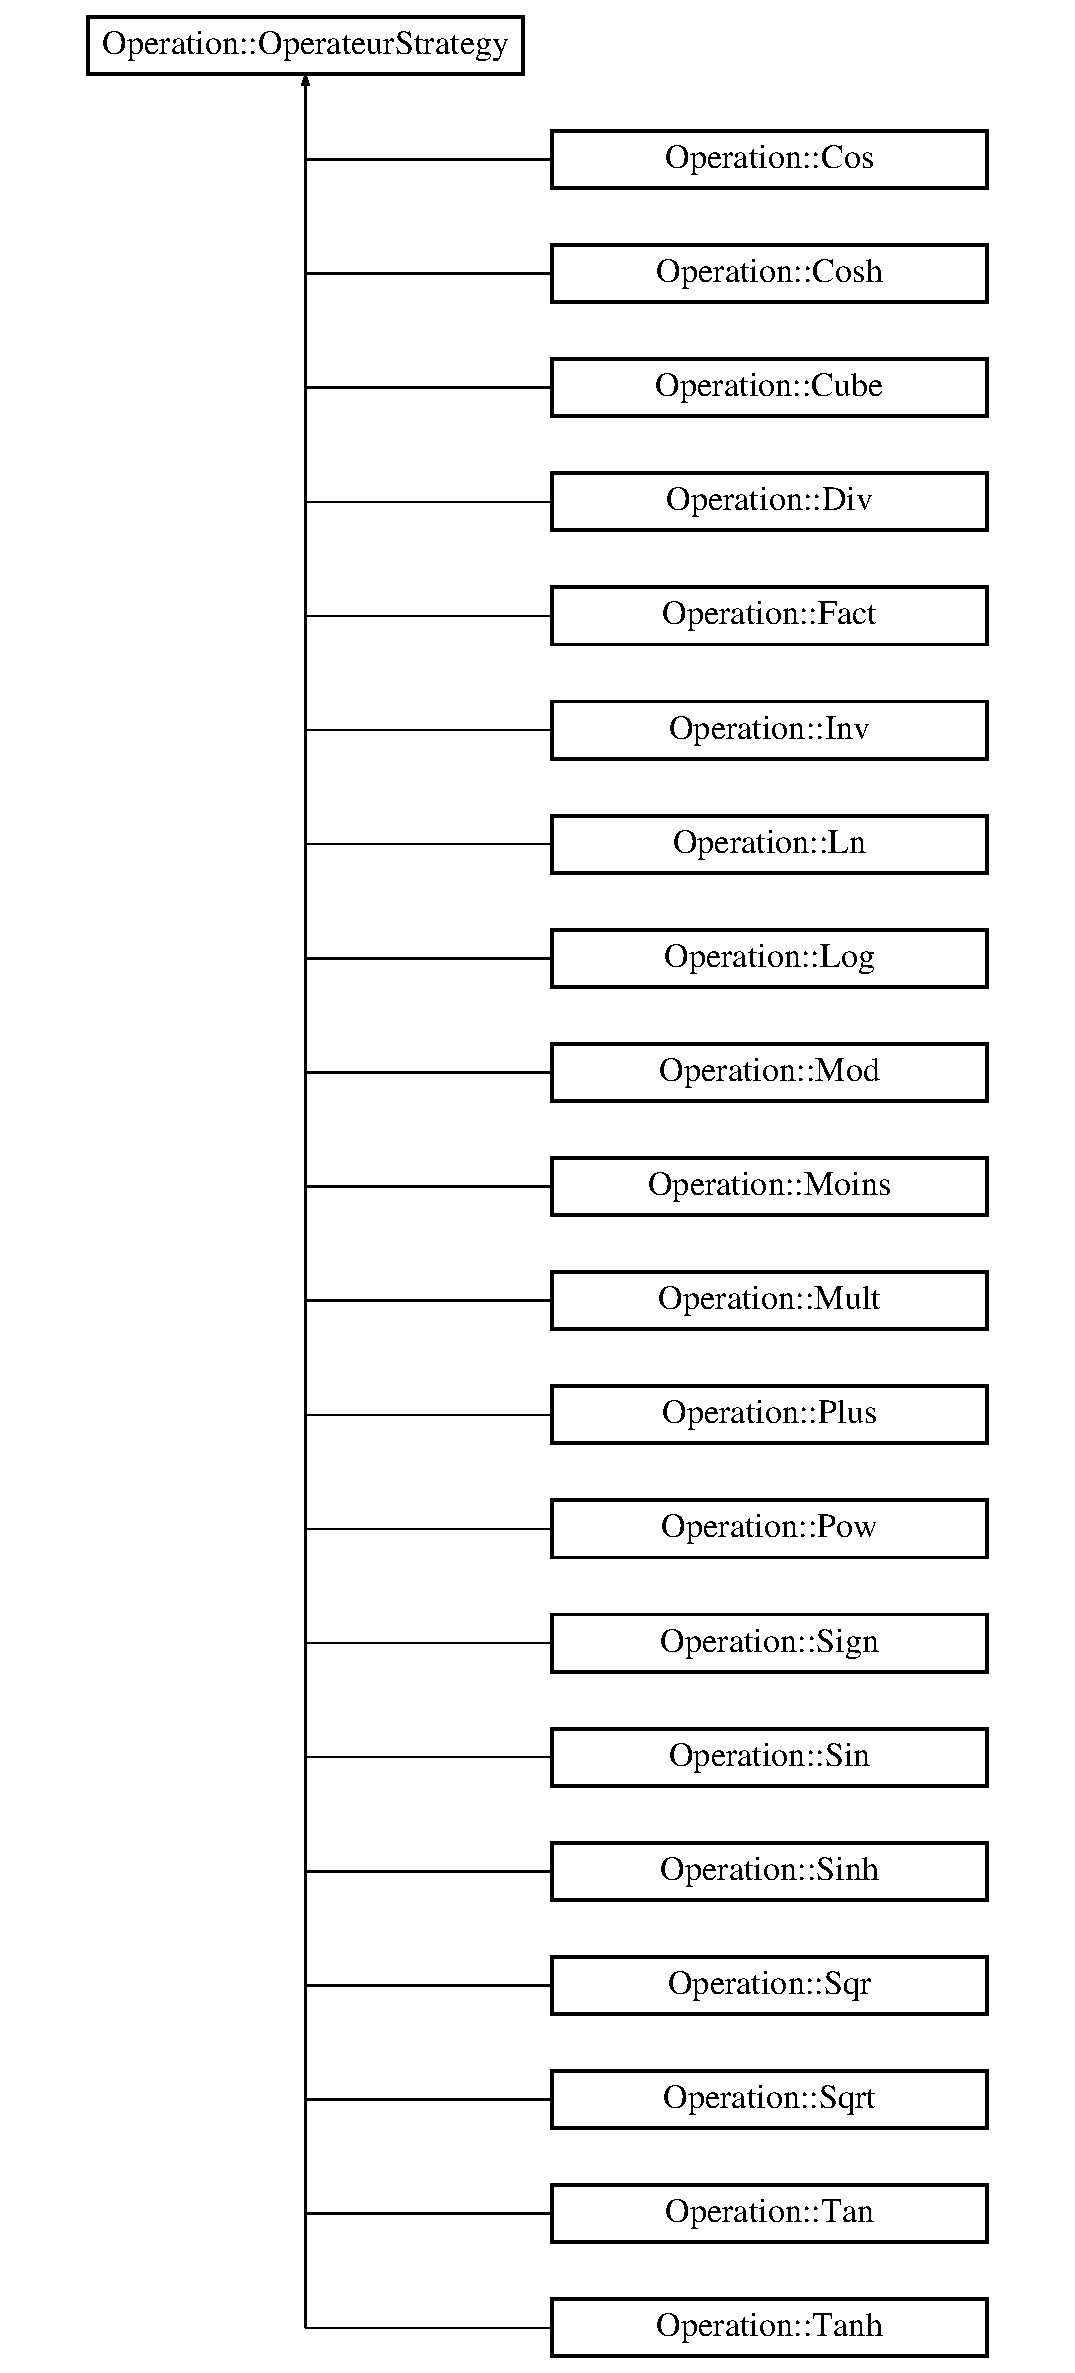
\includegraphics[height=12cm]{classOperation_1_1OperateurStrategy}
\end{center}
\end{figure}
\subsection*{Public Member Functions}
\begin{DoxyCompactItemize}
\item 
virtual \hyperlink{classNombre_1_1Data}{Data} \& \hyperlink{classOperation_1_1OperateurStrategy_a3a62ee4f37c773e8459f92c41b3127e1}{calcul} (\hyperlink{classPile}{Pile}$<$ \hyperlink{classNombre_1_1Data}{Data} $>$ \&p)=0
\begin{DoxyCompactList}\small\item\em permet d'effectuer le calcul et de mettre la pile à jour \item\end{DoxyCompactList}\end{DoxyCompactItemize}


\subsection{Detailed Description}
classe virtuelle dont hérite toutes les stratégies 

\subsection{Member Function Documentation}
\hypertarget{classOperation_1_1OperateurStrategy_a3a62ee4f37c773e8459f92c41b3127e1}{
\index{Operation::OperateurStrategy@{Operation::OperateurStrategy}!calcul@{calcul}}
\index{calcul@{calcul}!Operation::OperateurStrategy@{Operation::OperateurStrategy}}
\subsubsection[{calcul}]{\setlength{\rightskip}{0pt plus 5cm}virtual {\bf Data}\& Operation::OperateurStrategy::calcul ({\bf Pile}$<$ {\bf Data} $>$ \& {\em p})\hspace{0.3cm}{\ttfamily  \mbox{[}pure virtual\mbox{]}}}}
\label{classOperation_1_1OperateurStrategy_a3a62ee4f37c773e8459f92c41b3127e1}


permet d'effectuer le calcul et de mettre la pile à jour 


\begin{DoxyParams}{Parameters}
\item[{\em p}]: la pile à mettre à jour après calcul \end{DoxyParams}


The documentation for this class was generated from the following file:\begin{DoxyCompactItemize}
\item 
operateur.h\end{DoxyCompactItemize}

\hypertarget{classPile}{
\section{Pile$<$ T $>$ Class Template Reference}
\label{classPile}\index{Pile@{Pile}}
}


classe pile, gardant les données du programme  




{\ttfamily \#include $<$pile.h$>$}

Inheritance diagram for Pile$<$ T $>$:\begin{figure}[H]
\begin{center}
\leavevmode
\includegraphics[height=2cm]{classPile}
\end{center}
\end{figure}
\subsection*{Public Member Functions}
\begin{DoxyCompactItemize}
\item 
\hyperlink{classPile_a6393ea69d41a484a63f691bef44469a7}{Pile} ()
\begin{DoxyCompactList}\small\item\em Constructeur. \item\end{DoxyCompactList}\item 
\hyperlink{classPile_ac10aba315bae705a7821c41d5d31e11c}{$\sim$Pile} ()
\begin{DoxyCompactList}\small\item\em Destructeur. \item\end{DoxyCompactList}\item 
void \hyperlink{classPile_a685bd6ecb5c0c7805e4aa9f45e7a1289}{SWAP} (unsigned int x, unsigned int y)
\begin{DoxyCompactList}\small\item\em échange les éléments x et y de la pile. \item\end{DoxyCompactList}\item 
T \& \hyperlink{classPile_a35fc6cd5606215120f150629315c615a}{SUM} (const unsigned int x) const 
\begin{DoxyCompactList}\small\item\em Renvoie la Somme les x premiers elements de la pile. \item\end{DoxyCompactList}\item 
T \& \hyperlink{classPile_a5b576fb2729b6f1d79c05b8932b91588}{MEAN} (const unsigned int x) const 
\begin{DoxyCompactList}\small\item\em Renvoie la Moyenne des x premiers elements de la pile. \item\end{DoxyCompactList}\item 
\hypertarget{classPile_a0532e4cbf4f9521b09a30f5cd0f4f4ad}{
void \hyperlink{classPile_a0532e4cbf4f9521b09a30f5cd0f4f4ad}{CLEAR} ()}
\label{classPile_a0532e4cbf4f9521b09a30f5cd0f4f4ad}

\begin{DoxyCompactList}\small\item\em vide la pile \item\end{DoxyCompactList}\item 
\hypertarget{classPile_a8b4213827764783cb5b8463d81315055}{
void \hyperlink{classPile_a8b4213827764783cb5b8463d81315055}{DUP} () const }
\label{classPile_a8b4213827764783cb5b8463d81315055}

\begin{DoxyCompactList}\small\item\em Duplique le premier element de la pile. \item\end{DoxyCompactList}\item 
\hypertarget{classPile_ab3bff8336491d068c21958939737571f}{
void \hyperlink{classPile_ab3bff8336491d068c21958939737571f}{DROP} ()}
\label{classPile_ab3bff8336491d068c21958939737571f}

\begin{DoxyCompactList}\small\item\em libère le premier element de la pile \item\end{DoxyCompactList}\item 
\hypertarget{classPile_a0615cbdce400a7aea271de2193e46fe4}{
\hyperlink{classPile}{Pile}$<$ T $>$ \& \hyperlink{classPile_a0615cbdce400a7aea271de2193e46fe4}{clone} ()}
\label{classPile_a0615cbdce400a7aea271de2193e46fe4}

\begin{DoxyCompactList}\small\item\em Renvoie une reference vers une copie de la pile. \item\end{DoxyCompactList}\item 
void \hyperlink{classPile_a5e80dbc7bc37bb4cc6439a2299bb2327}{addPile} (T $\ast$x)
\begin{DoxyCompactList}\small\item\em Ajoute un element dans la pile. \item\end{DoxyCompactList}\item 
\hypertarget{classPile_a3e8bd308a162809611df5e2872946820}{
int \hyperlink{classPile_a3e8bd308a162809611df5e2872946820}{taille} ()}
\label{classPile_a3e8bd308a162809611df5e2872946820}

\begin{DoxyCompactList}\small\item\em retourne la taille de la pile \item\end{DoxyCompactList}\item 
\hypertarget{classPile_ac3e83355eb3e97f68e1a91e90ee09123}{
\hyperlink{classPile}{Pile}$<$ T $>$ \& \hyperlink{classPile_ac3e83355eb3e97f68e1a91e90ee09123}{pileResultat} () const }
\label{classPile_ac3e83355eb3e97f68e1a91e90ee09123}

\begin{DoxyCompactList}\small\item\em retourne les resultats seulement dans la pile de stockage \item\end{DoxyCompactList}\end{DoxyCompactItemize}


\subsection{Detailed Description}
\subsubsection*{template$<$typename T$>$ class Pile$<$ T $>$}

classe pile, gardant les données du programme 

\subsection{Constructor \& Destructor Documentation}
\hypertarget{classPile_a6393ea69d41a484a63f691bef44469a7}{
\index{Pile@{Pile}!Pile@{Pile}}
\index{Pile@{Pile}!Pile@{Pile}}
\subsubsection[{Pile}]{\setlength{\rightskip}{0pt plus 5cm}template$<$typename T$>$ {\bf Pile}$<$ T $>$::{\bf Pile} ()\hspace{0.3cm}{\ttfamily  \mbox{[}inline\mbox{]}}}}
\label{classPile_a6393ea69d41a484a63f691bef44469a7}


Constructeur. 

Constructeur de la classe \hyperlink{classPile}{Pile}, sans argument \hypertarget{classPile_ac10aba315bae705a7821c41d5d31e11c}{
\index{Pile@{Pile}!$\sim$Pile@{$\sim$Pile}}
\index{$\sim$Pile@{$\sim$Pile}!Pile@{Pile}}
\subsubsection[{$\sim$Pile}]{\setlength{\rightskip}{0pt plus 5cm}template$<$typename T$>$ {\bf Pile}$<$ T $>$::$\sim${\bf Pile} ()\hspace{0.3cm}{\ttfamily  \mbox{[}inline\mbox{]}}}}
\label{classPile_ac10aba315bae705a7821c41d5d31e11c}


Destructeur. 

Destructeur de la classe \hyperlink{classPile}{Pile}, appelle le destructeur de chaque élément 

\subsection{Member Function Documentation}
\hypertarget{classPile_a5e80dbc7bc37bb4cc6439a2299bb2327}{
\index{Pile@{Pile}!addPile@{addPile}}
\index{addPile@{addPile}!Pile@{Pile}}
\subsubsection[{addPile}]{\setlength{\rightskip}{0pt plus 5cm}template$<$typename T$>$ void {\bf Pile}$<$ T $>$::addPile (T $\ast$ {\em x})\hspace{0.3cm}{\ttfamily  \mbox{[}inline\mbox{]}}}}
\label{classPile_a5e80dbc7bc37bb4cc6439a2299bb2327}


Ajoute un element dans la pile. 


\begin{DoxyParams}{Parameters}
\item[{\em x}]: élément à ajouter \end{DoxyParams}
\hypertarget{classPile_a5b576fb2729b6f1d79c05b8932b91588}{
\index{Pile@{Pile}!MEAN@{MEAN}}
\index{MEAN@{MEAN}!Pile@{Pile}}
\subsubsection[{MEAN}]{\setlength{\rightskip}{0pt plus 5cm}template$<$typename T $>$ T \& {\bf Pile}$<$ T $>$::MEAN (const unsigned int {\em x}) const\hspace{0.3cm}{\ttfamily  \mbox{[}inline\mbox{]}}}}
\label{classPile_a5b576fb2729b6f1d79c05b8932b91588}


Renvoie la Moyenne des x premiers elements de la pile. 


\begin{DoxyParams}{Parameters}
\item[{\em x}]: nombre d'éléments à sommer puis à faire la moyenne \end{DoxyParams}
\hypertarget{classPile_a35fc6cd5606215120f150629315c615a}{
\index{Pile@{Pile}!SUM@{SUM}}
\index{SUM@{SUM}!Pile@{Pile}}
\subsubsection[{SUM}]{\setlength{\rightskip}{0pt plus 5cm}template$<$typename T $>$ T \& {\bf Pile}$<$ T $>$::SUM (const unsigned int {\em x}) const\hspace{0.3cm}{\ttfamily  \mbox{[}inline\mbox{]}}}}
\label{classPile_a35fc6cd5606215120f150629315c615a}


Renvoie la Somme les x premiers elements de la pile. 


\begin{DoxyParams}{Parameters}
\item[{\em x}]: nombre d'éléments à sommer \end{DoxyParams}
\hypertarget{classPile_a685bd6ecb5c0c7805e4aa9f45e7a1289}{
\index{Pile@{Pile}!SWAP@{SWAP}}
\index{SWAP@{SWAP}!Pile@{Pile}}
\subsubsection[{SWAP}]{\setlength{\rightskip}{0pt plus 5cm}template$<$typename T $>$ void {\bf Pile}$<$ T $>$::SWAP (unsigned int {\em x}, \/  unsigned int {\em y})\hspace{0.3cm}{\ttfamily  \mbox{[}inline\mbox{]}}}}
\label{classPile_a685bd6ecb5c0c7805e4aa9f45e7a1289}


échange les éléments x et y de la pile. 


\begin{DoxyParams}{Parameters}
\item[{\em x}]: élément de position x dans la pile \item[{\em y}]: élément de position y dans la pile \end{DoxyParams}


The documentation for this class was generated from the following files:\begin{DoxyCompactItemize}
\item 
pile.h\item 
pile.cpp\end{DoxyCompactItemize}

\hypertarget{classOperation_1_1Plus}{
\section{Operation::Plus Class Reference}
\label{classOperation_1_1Plus}\index{Operation::Plus@{Operation::Plus}}
}


classe permettant d'effectuer l'opération plus  




{\ttfamily \#include $<$operateur.h$>$}

Inheritance diagram for Operation::Plus:\begin{figure}[H]
\begin{center}
\leavevmode
\includegraphics[height=2cm]{classOperation_1_1Plus}
\end{center}
\end{figure}
\subsection*{Public Member Functions}
\begin{DoxyCompactItemize}
\item 
\hyperlink{classNombre_1_1Data}{Data} \& \hyperlink{classOperation_1_1Plus_ad497644da3ea64318f15777d1e3ddcc9}{calcul} (\hyperlink{classPile}{Pile}$<$ \hyperlink{classNombre_1_1Data}{Data} $>$ $\ast$p)
\begin{DoxyCompactList}\small\item\em permet d'effectuer le calcul et de mettre la pile à jour \item\end{DoxyCompactList}\item 
\hyperlink{classNombre_1_1Complexe}{Complexe} \& \hyperlink{classOperation_1_1Plus_aa80c86b918fd8e37d08ea892d3704596}{plusComplexe} (const \hyperlink{classNombre_1_1Complexe}{Complexe} \&a, const \hyperlink{classNombre_1_1Complexe}{Complexe} \&b)
\begin{DoxyCompactList}\small\item\em permet d'effectuer l'opération plus pour deux complexes \item\end{DoxyCompactList}\item 
\hyperlink{classNombre_1_1Rationnel}{Rationnel} \& \hyperlink{classOperation_1_1Plus_adb1aba33aad17c96c1d9b5624e8df22e}{plusRationnel} (const \hyperlink{classNombre_1_1Rationnel}{Rationnel} \&r1, const \hyperlink{classNombre_1_1Rationnel}{Rationnel} \&r2)
\begin{DoxyCompactList}\small\item\em permet d'effectuer l'opération plus pour deux rationnels \item\end{DoxyCompactList}\end{DoxyCompactItemize}


\subsection{Detailed Description}
classe permettant d'effectuer l'opération plus 

\subsection{Member Function Documentation}
\hypertarget{classOperation_1_1Plus_ad497644da3ea64318f15777d1e3ddcc9}{
\index{Operation::Plus@{Operation::Plus}!calcul@{calcul}}
\index{calcul@{calcul}!Operation::Plus@{Operation::Plus}}
\subsubsection[{calcul}]{\setlength{\rightskip}{0pt plus 5cm}{\bf Data} \& Operation::Plus::calcul ({\bf Pile}$<$ {\bf Data} $>$ $\ast$ {\em p})}}
\label{classOperation_1_1Plus_ad497644da3ea64318f15777d1e3ddcc9}


permet d'effectuer le calcul et de mettre la pile à jour 


\begin{DoxyParams}{Parameters}
\item[{\em p}]: la pile à mettre à jour après calcul \end{DoxyParams}
\hypertarget{classOperation_1_1Plus_aa80c86b918fd8e37d08ea892d3704596}{
\index{Operation::Plus@{Operation::Plus}!plusComplexe@{plusComplexe}}
\index{plusComplexe@{plusComplexe}!Operation::Plus@{Operation::Plus}}
\subsubsection[{plusComplexe}]{\setlength{\rightskip}{0pt plus 5cm}{\bf Complexe} \& Operation::Plus::plusComplexe (const {\bf Complexe} \& {\em a}, \/  const {\bf Complexe} \& {\em b})}}
\label{classOperation_1_1Plus_aa80c86b918fd8e37d08ea892d3704596}


permet d'effectuer l'opération plus pour deux complexes 


\begin{DoxyParams}{Parameters}
\item[{\em a}]: le premier complexe \item[{\em b}]: le second complexe \end{DoxyParams}
\hypertarget{classOperation_1_1Plus_adb1aba33aad17c96c1d9b5624e8df22e}{
\index{Operation::Plus@{Operation::Plus}!plusRationnel@{plusRationnel}}
\index{plusRationnel@{plusRationnel}!Operation::Plus@{Operation::Plus}}
\subsubsection[{plusRationnel}]{\setlength{\rightskip}{0pt plus 5cm}{\bf Rationnel} \& Operation::Plus::plusRationnel (const {\bf Rationnel} \& {\em r1}, \/  const {\bf Rationnel} \& {\em r2})}}
\label{classOperation_1_1Plus_adb1aba33aad17c96c1d9b5624e8df22e}


permet d'effectuer l'opération plus pour deux rationnels 


\begin{DoxyParams}{Parameters}
\item[{\em r1}]: le premier rationnel \item[{\em r2}]: le second rationnel \end{DoxyParams}


The documentation for this class was generated from the following files:\begin{DoxyCompactItemize}
\item 
operateur.h\item 
operateur.cpp\end{DoxyCompactItemize}

\hypertarget{classOperation_1_1Pow}{
\section{Operation::Pow Class Reference}
\label{classOperation_1_1Pow}\index{Operation::Pow@{Operation::Pow}}
}


classe permettant d'effectuer l'opération pow  




{\ttfamily \#include $<$operateur.h$>$}

Inheritance diagram for Operation::Pow:\begin{figure}[H]
\begin{center}
\leavevmode
\includegraphics[height=2cm]{classOperation_1_1Pow}
\end{center}
\end{figure}
\subsection*{Public Member Functions}
\begin{DoxyCompactItemize}
\item 
\hyperlink{classNombre_1_1Data}{Data} \& \hyperlink{classOperation_1_1Pow_a11a1d7683969a9b487debfaeecd065c4}{calcul} (\hyperlink{classPile}{Pile}$<$ \hyperlink{classNombre_1_1Data}{Data} $>$ $\ast$p)
\begin{DoxyCompactList}\small\item\em permet d'effectuer le calcul et de mettre la pile à jour \item\end{DoxyCompactList}\end{DoxyCompactItemize}


\subsection{Detailed Description}
classe permettant d'effectuer l'opération pow 

\subsection{Member Function Documentation}
\hypertarget{classOperation_1_1Pow_a11a1d7683969a9b487debfaeecd065c4}{
\index{Operation::Pow@{Operation::Pow}!calcul@{calcul}}
\index{calcul@{calcul}!Operation::Pow@{Operation::Pow}}
\subsubsection[{calcul}]{\setlength{\rightskip}{0pt plus 5cm}{\bf Data}\& Operation::Pow::calcul ({\bf Pile}$<$ {\bf Data} $>$ $\ast$ {\em p})}}
\label{classOperation_1_1Pow_a11a1d7683969a9b487debfaeecd065c4}


permet d'effectuer le calcul et de mettre la pile à jour 


\begin{DoxyParams}{Parameters}
\item[{\em p}]: la pile à mettre à jour après calcul \end{DoxyParams}


The documentation for this class was generated from the following file:\begin{DoxyCompactItemize}
\item 
operateur.h\end{DoxyCompactItemize}

\hypertarget{classQStack}{
\section{QStack Class Reference}
\label{classQStack}\index{QStack@{QStack}}
}
Inheritance diagram for QStack:\begin{figure}[H]
\begin{center}
\leavevmode
\includegraphics[height=2cm]{classQStack}
\end{center}
\end{figure}


The documentation for this class was generated from the following file:\begin{DoxyCompactItemize}
\item 
pile.h\end{DoxyCompactItemize}

\hypertarget{classNombre_1_1Rationnel}{
\section{Nombre::Rationnel Class Reference}
\label{classNombre_1_1Rationnel}\index{Nombre::Rationnel@{Nombre::Rationnel}}
}


classe représentant les nombres rationnels  




{\ttfamily \#include $<$data.h$>$}

Inheritance diagram for Nombre::Rationnel:\begin{figure}[H]
\begin{center}
\leavevmode
\includegraphics[height=3cm]{classNombre_1_1Rationnel}
\end{center}
\end{figure}
\subsection*{Public Member Functions}
\begin{DoxyCompactItemize}
\item 
\hyperlink{classNombre_1_1Rationnel_ab0ee4363dc90feacdc79b0c78929059a}{Rationnel} (int n, int d)
\begin{DoxyCompactList}\small\item\em Constructeur. \item\end{DoxyCompactList}\item 
\hyperlink{classNombre_1_1Rationnel_a6271bc256512bcd61dfb7a671f6af90e}{Rationnel} (const \hyperlink{classNombre_1_1Rationnel}{Rationnel} \&e)
\begin{DoxyCompactList}\small\item\em Constructeur par recopie. \item\end{DoxyCompactList}\item 
\hyperlink{classNombre_1_1Rationnel_a9ceaf1d936e80578441fdd95181932eb}{Rationnel} (const QString \&s)
\begin{DoxyCompactList}\small\item\em Constructeur. \item\end{DoxyCompactList}\item 
\hyperlink{classNombre_1_1Rationnel_a436ac28026acabc38547f594c07ad6dd}{$\sim$Rationnel} ()
\begin{DoxyCompactList}\small\item\em Destructeur. \item\end{DoxyCompactList}\item 
\hypertarget{classNombre_1_1Rationnel_a87e5a70d65efb04d24e4501c49e93793}{
\hyperlink{classNombre_1_1Entier}{Entier} \& \hyperlink{classNombre_1_1Rationnel_a87e5a70d65efb04d24e4501c49e93793}{getNumerateur} () const }
\label{classNombre_1_1Rationnel_a87e5a70d65efb04d24e4501c49e93793}

\begin{DoxyCompactList}\small\item\em retourne le numerateur \item\end{DoxyCompactList}\item 
\hypertarget{classNombre_1_1Rationnel_a7c3f2070efba44aa67ea1c4fe8c22704}{
\hyperlink{classNombre_1_1Entier}{Entier} \& \hyperlink{classNombre_1_1Rationnel_a7c3f2070efba44aa67ea1c4fe8c22704}{getDenominateur} () const }
\label{classNombre_1_1Rationnel_a7c3f2070efba44aa67ea1c4fe8c22704}

\begin{DoxyCompactList}\small\item\em retourne le denominateur \item\end{DoxyCompactList}\item 
void \hyperlink{classNombre_1_1Rationnel_a18c8f925fd5d353e8b985c9ea725fb70}{setNumerateur} (int n)
\begin{DoxyCompactList}\small\item\em change le numerateur \item\end{DoxyCompactList}\item 
void \hyperlink{classNombre_1_1Rationnel_abe4d3136a4e1aa0d76575602d6e4630f}{setDenominateur} (int d)
\begin{DoxyCompactList}\small\item\em change le denominateur \item\end{DoxyCompactList}\item 
\hypertarget{classNombre_1_1Rationnel_a12ee060e5fca5f4291b222983d727268}{
void \hyperlink{classNombre_1_1Rationnel_a12ee060e5fca5f4291b222983d727268}{simplifier} ()}
\label{classNombre_1_1Rationnel_a12ee060e5fca5f4291b222983d727268}

\begin{DoxyCompactList}\small\item\em simplifie le rationnel en utilisant le pvcd \item\end{DoxyCompactList}\item 
\hypertarget{classNombre_1_1Rationnel_ae6cf0b5b3c8a7146f4f1d21a80f34397}{
\hyperlink{classNombre_1_1Rationnel}{Rationnel} \& \hyperlink{classNombre_1_1Rationnel_ae6cf0b5b3c8a7146f4f1d21a80f34397}{toRationnel} () const }
\label{classNombre_1_1Rationnel_ae6cf0b5b3c8a7146f4f1d21a80f34397}

\begin{DoxyCompactList}\small\item\em transforme la \hyperlink{classNombre_1_1Data}{Data} en \hyperlink{classNombre_1_1Rationnel}{Rationnel} \item\end{DoxyCompactList}\item 
\hypertarget{classNombre_1_1Rationnel_a441c5df2959c34f0253d40770467a2ed}{
\hyperlink{classNombre_1_1Entier}{Entier} \& \hyperlink{classNombre_1_1Rationnel_a441c5df2959c34f0253d40770467a2ed}{toEntier} () const }
\label{classNombre_1_1Rationnel_a441c5df2959c34f0253d40770467a2ed}

\begin{DoxyCompactList}\small\item\em transforme la \hyperlink{classNombre_1_1Data}{Data} en \hyperlink{classNombre_1_1Entier}{Entier} \item\end{DoxyCompactList}\item 
\hypertarget{classNombre_1_1Rationnel_a81f1f8f07b7b896ceaa00d4da2461c98}{
\hyperlink{classNombre_1_1Reel}{Reel} \& \hyperlink{classNombre_1_1Rationnel_a81f1f8f07b7b896ceaa00d4da2461c98}{toReel} () const }
\label{classNombre_1_1Rationnel_a81f1f8f07b7b896ceaa00d4da2461c98}

\begin{DoxyCompactList}\small\item\em transforme la \hyperlink{classNombre_1_1Data}{Data} en \hyperlink{classNombre_1_1Reel}{Reel} \item\end{DoxyCompactList}\item 
\hyperlink{classNombre_1_1Entier}{Entier} \hyperlink{classNombre_1_1Rationnel_a887d49ae935aa401e0dcce5c8534b894}{pgcd} (const \hyperlink{classNombre_1_1Entier}{Entier} \&a, const \hyperlink{classNombre_1_1Entier}{Entier} \&b)
\begin{DoxyCompactList}\small\item\em retourne le pvcd \item\end{DoxyCompactList}\item 
\hypertarget{classNombre_1_1Rationnel_a2631c49cbe0ecd80076a274d6c68cc28}{
QString \& \hyperlink{classNombre_1_1Rationnel_a2631c49cbe0ecd80076a274d6c68cc28}{toString} () const }
\label{classNombre_1_1Rationnel_a2631c49cbe0ecd80076a274d6c68cc28}

\begin{DoxyCompactList}\small\item\em renvoie l'information en QString de la classe \item\end{DoxyCompactList}\item 
\hypertarget{classNombre_1_1Rationnel_a982e0d69944eb578cd5d168e11559ab0}{
\hyperlink{classNombre_1_1Rationnel}{Rationnel} \& \hyperlink{classNombre_1_1Rationnel_a982e0d69944eb578cd5d168e11559ab0}{clone} () const }
\label{classNombre_1_1Rationnel_a982e0d69944eb578cd5d168e11559ab0}

\begin{DoxyCompactList}\small\item\em clone la classe \item\end{DoxyCompactList}\end{DoxyCompactItemize}
\subsection*{Static Public Member Functions}
\begin{DoxyCompactItemize}
\item 
static bool \hyperlink{classNombre_1_1Rationnel_a4c6e7150cba3e9ab182361072965f209}{isRationnel} (const QString \&s)
\begin{DoxyCompactList}\small\item\em test si une string est un rationnel \item\end{DoxyCompactList}\end{DoxyCompactItemize}


\subsection{Detailed Description}
classe représentant les nombres rationnels 

\subsection{Constructor \& Destructor Documentation}
\hypertarget{classNombre_1_1Rationnel_ab0ee4363dc90feacdc79b0c78929059a}{
\index{Nombre::Rationnel@{Nombre::Rationnel}!Rationnel@{Rationnel}}
\index{Rationnel@{Rationnel}!Nombre::Rationnel@{Nombre::Rationnel}}
\subsubsection[{Rationnel}]{\setlength{\rightskip}{0pt plus 5cm}Nombre::Rationnel::Rationnel (int {\em n}, \/  int {\em d})\hspace{0.3cm}{\ttfamily  \mbox{[}inline\mbox{]}}}}
\label{classNombre_1_1Rationnel_ab0ee4363dc90feacdc79b0c78929059a}


Constructeur. 

Constructeur de la classe


\begin{DoxyParams}{Parameters}
\item[{\em n}]: numerateur \item[{\em d}]: denominateur \end{DoxyParams}
\hypertarget{classNombre_1_1Rationnel_a6271bc256512bcd61dfb7a671f6af90e}{
\index{Nombre::Rationnel@{Nombre::Rationnel}!Rationnel@{Rationnel}}
\index{Rationnel@{Rationnel}!Nombre::Rationnel@{Nombre::Rationnel}}
\subsubsection[{Rationnel}]{\setlength{\rightskip}{0pt plus 5cm}Nombre::Rationnel::Rationnel (const {\bf Rationnel} \& {\em e})\hspace{0.3cm}{\ttfamily  \mbox{[}inline\mbox{]}}}}
\label{classNombre_1_1Rationnel_a6271bc256512bcd61dfb7a671f6af90e}


Constructeur par recopie. 

Constructeur de la classe


\begin{DoxyParams}{Parameters}
\item[{\em e}]: rationnel à copier \end{DoxyParams}
\hypertarget{classNombre_1_1Rationnel_a9ceaf1d936e80578441fdd95181932eb}{
\index{Nombre::Rationnel@{Nombre::Rationnel}!Rationnel@{Rationnel}}
\index{Rationnel@{Rationnel}!Nombre::Rationnel@{Nombre::Rationnel}}
\subsubsection[{Rationnel}]{\setlength{\rightskip}{0pt plus 5cm}Nombre::Rationnel::Rationnel (const QString \& {\em s})\hspace{0.3cm}{\ttfamily  \mbox{[}inline\mbox{]}}}}
\label{classNombre_1_1Rationnel_a9ceaf1d936e80578441fdd95181932eb}


Constructeur. 

Constructeur de la classe


\begin{DoxyParams}{Parameters}
\item[{\em s}]: qstring ayant la valeur du rationnel \end{DoxyParams}
\hypertarget{classNombre_1_1Rationnel_a436ac28026acabc38547f594c07ad6dd}{
\index{Nombre::Rationnel@{Nombre::Rationnel}!$\sim$Rationnel@{$\sim$Rationnel}}
\index{$\sim$Rationnel@{$\sim$Rationnel}!Nombre::Rationnel@{Nombre::Rationnel}}
\subsubsection[{$\sim$Rationnel}]{\setlength{\rightskip}{0pt plus 5cm}Nombre::Rationnel::$\sim$Rationnel ()\hspace{0.3cm}{\ttfamily  \mbox{[}inline\mbox{]}}}}
\label{classNombre_1_1Rationnel_a436ac28026acabc38547f594c07ad6dd}


Destructeur. 

Destructeur de la classe 

\subsection{Member Function Documentation}
\hypertarget{classNombre_1_1Rationnel_a4c6e7150cba3e9ab182361072965f209}{
\index{Nombre::Rationnel@{Nombre::Rationnel}!isRationnel@{isRationnel}}
\index{isRationnel@{isRationnel}!Nombre::Rationnel@{Nombre::Rationnel}}
\subsubsection[{isRationnel}]{\setlength{\rightskip}{0pt plus 5cm}bool Nombre::Rationnel::isRationnel (const QString \& {\em s})\hspace{0.3cm}{\ttfamily  \mbox{[}static\mbox{]}}}}
\label{classNombre_1_1Rationnel_a4c6e7150cba3e9ab182361072965f209}


test si une string est un rationnel 


\begin{DoxyParams}{Parameters}
\item[{\em s}]: la QString a tester \end{DoxyParams}
\hypertarget{classNombre_1_1Rationnel_a887d49ae935aa401e0dcce5c8534b894}{
\index{Nombre::Rationnel@{Nombre::Rationnel}!pgcd@{pgcd}}
\index{pgcd@{pgcd}!Nombre::Rationnel@{Nombre::Rationnel}}
\subsubsection[{pgcd}]{\setlength{\rightskip}{0pt plus 5cm}{\bf Entier} Rationnel::pgcd (const {\bf Entier} \& {\em a}, \/  const {\bf Entier} \& {\em b})}}
\label{classNombre_1_1Rationnel_a887d49ae935aa401e0dcce5c8534b894}


retourne le pvcd 


\begin{DoxyParams}{Parameters}
\item[{\em a}]: entier a \item[{\em b}]: entier b \end{DoxyParams}
\hypertarget{classNombre_1_1Rationnel_abe4d3136a4e1aa0d76575602d6e4630f}{
\index{Nombre::Rationnel@{Nombre::Rationnel}!setDenominateur@{setDenominateur}}
\index{setDenominateur@{setDenominateur}!Nombre::Rationnel@{Nombre::Rationnel}}
\subsubsection[{setDenominateur}]{\setlength{\rightskip}{0pt plus 5cm}void Nombre::Rationnel::setDenominateur (int {\em d})\hspace{0.3cm}{\ttfamily  \mbox{[}inline\mbox{]}}}}
\label{classNombre_1_1Rationnel_abe4d3136a4e1aa0d76575602d6e4630f}


change le denominateur 


\begin{DoxyParams}{Parameters}
\item[{\em d}]: nouvelle valeur \end{DoxyParams}
\hypertarget{classNombre_1_1Rationnel_a18c8f925fd5d353e8b985c9ea725fb70}{
\index{Nombre::Rationnel@{Nombre::Rationnel}!setNumerateur@{setNumerateur}}
\index{setNumerateur@{setNumerateur}!Nombre::Rationnel@{Nombre::Rationnel}}
\subsubsection[{setNumerateur}]{\setlength{\rightskip}{0pt plus 5cm}void Nombre::Rationnel::setNumerateur (int {\em n})\hspace{0.3cm}{\ttfamily  \mbox{[}inline\mbox{]}}}}
\label{classNombre_1_1Rationnel_a18c8f925fd5d353e8b985c9ea725fb70}


change le numerateur 


\begin{DoxyParams}{Parameters}
\item[{\em n}]: nouvelle valeur \end{DoxyParams}


The documentation for this class was generated from the following files:\begin{DoxyCompactItemize}
\item 
data.h\item 
data.cpp\end{DoxyCompactItemize}

\hypertarget{classRationnelFactory}{
\section{RationnelFactory Class Reference}
\label{classRationnelFactory}\index{RationnelFactory@{RationnelFactory}}
}


classe gérant la création des Rationnel  




{\ttfamily \#include $<$factory.h$>$}

Inheritance diagram for RationnelFactory:\begin{figure}[H]
\begin{center}
\leavevmode
\includegraphics[height=2cm]{classRationnelFactory}
\end{center}
\end{figure}
\subsection*{Static Public Member Functions}
\begin{DoxyCompactItemize}
\item 
static \hyperlink{classNombre_1_1Rationnel}{Nombre::Rationnel} \& \hyperlink{classRationnelFactory_aefce747781195682e508436186875fca}{creer} (QString s)
\begin{DoxyCompactList}\small\item\em cree une nouvelle Data à partir d'une QString et la renvoie \item\end{DoxyCompactList}\end{DoxyCompactItemize}


\subsection{Detailed Description}
classe gérant la création des Rationnel 

\subsection{Member Function Documentation}
\hypertarget{classRationnelFactory_aefce747781195682e508436186875fca}{
\index{RationnelFactory@{RationnelFactory}!creer@{creer}}
\index{creer@{creer}!RationnelFactory@{RationnelFactory}}
\subsubsection[{creer}]{\setlength{\rightskip}{0pt plus 5cm}{\bf Rationnel} \& RationnelFactory::creer (QString {\em s})\hspace{0.3cm}{\ttfamily  \mbox{[}static\mbox{]}}}}
\label{classRationnelFactory_aefce747781195682e508436186875fca}


cree une nouvelle Data à partir d'une QString et la renvoie 


\begin{DoxyParams}{Parameters}
\item[{\em s}]: QString servant de base à la création de la donnée \end{DoxyParams}


Reimplemented from \hyperlink{classFactory_afe37851e80172944b37491a952a28370}{Factory}.



The documentation for this class was generated from the following files:\begin{DoxyCompactItemize}
\item 
factory.h\item 
factory.cpp\end{DoxyCompactItemize}

\hypertarget{classNombre_1_1Reel}{
\section{Nombre::Reel Class Reference}
\label{classNombre_1_1Reel}\index{Nombre::Reel@{Nombre::Reel}}
}


classe représentant les nombres réels  




{\ttfamily \#include $<$data.h$>$}

Inheritance diagram for Nombre::Reel:\begin{figure}[H]
\begin{center}
\leavevmode
\includegraphics[height=3cm]{classNombre_1_1Reel}
\end{center}
\end{figure}
\subsection*{Public Member Functions}
\begin{DoxyCompactItemize}
\item 
\hyperlink{classNombre_1_1Reel_a7435c6c760397d4a481e5f8a684da18d}{Reel} (double d)
\begin{DoxyCompactList}\small\item\em Constructeur. \item\end{DoxyCompactList}\item 
\hyperlink{classNombre_1_1Reel_a4343cb0e3dc44c60a4a6239da218b196}{Reel} (const \hyperlink{classNombre_1_1Reel}{Reel} \&e)
\begin{DoxyCompactList}\small\item\em Constructeur par recopie. \item\end{DoxyCompactList}\item 
\hyperlink{classNombre_1_1Reel_a810be76247a67b0bcea16e94bc734fc2}{Reel} (const QString \&s)
\begin{DoxyCompactList}\small\item\em Constructeur. \item\end{DoxyCompactList}\item 
\hypertarget{classNombre_1_1Reel_afa1b08befdd635d236ee485df5d39574}{
double \hyperlink{classNombre_1_1Reel_afa1b08befdd635d236ee485df5d39574}{getValeur} () const }
\label{classNombre_1_1Reel_afa1b08befdd635d236ee485df5d39574}

\begin{DoxyCompactList}\small\item\em retourne la valeur du réel \item\end{DoxyCompactList}\item 
void \hyperlink{classNombre_1_1Reel_a7c8c6736be61f1bb9583bb2f67310d24}{setValeur} (double v)
\begin{DoxyCompactList}\small\item\em change la valeur du réel \item\end{DoxyCompactList}\item 
\hypertarget{classNombre_1_1Reel_a199da1c39952cf57288d594dc216050a}{
\hyperlink{classNombre_1_1Reel}{Reel} \& \hyperlink{classNombre_1_1Reel_a199da1c39952cf57288d594dc216050a}{toReel} () const }
\label{classNombre_1_1Reel_a199da1c39952cf57288d594dc216050a}

\begin{DoxyCompactList}\small\item\em transforme la \hyperlink{classNombre_1_1Data}{Data} en \hyperlink{classNombre_1_1Reel}{Reel} \item\end{DoxyCompactList}\item 
\hypertarget{classNombre_1_1Reel_ae72c1aae90cae815491ccc6fc67b74a4}{
\hyperlink{classNombre_1_1Entier}{Entier} \& \hyperlink{classNombre_1_1Reel_ae72c1aae90cae815491ccc6fc67b74a4}{toEntier} () const }
\label{classNombre_1_1Reel_ae72c1aae90cae815491ccc6fc67b74a4}

\begin{DoxyCompactList}\small\item\em transforme la \hyperlink{classNombre_1_1Data}{Data} en \hyperlink{classNombre_1_1Entier}{Entier} \item\end{DoxyCompactList}\item 
\hypertarget{classNombre_1_1Reel_a2cd0dce1eb92158ba79bd8762bafbc12}{
\hyperlink{classNombre_1_1Rationnel}{Rationnel} \& \hyperlink{classNombre_1_1Reel_a2cd0dce1eb92158ba79bd8762bafbc12}{toRationnel} () const }
\label{classNombre_1_1Reel_a2cd0dce1eb92158ba79bd8762bafbc12}

\begin{DoxyCompactList}\small\item\em transforme la \hyperlink{classNombre_1_1Data}{Data} en \hyperlink{classNombre_1_1Rationnel}{Rationnel} \item\end{DoxyCompactList}\item 
\hypertarget{classNombre_1_1Reel_a21b53eb0c5fce7a2fd84ffd7ad0a1086}{
QString \& \hyperlink{classNombre_1_1Reel_a21b53eb0c5fce7a2fd84ffd7ad0a1086}{toString} () const }
\label{classNombre_1_1Reel_a21b53eb0c5fce7a2fd84ffd7ad0a1086}

\begin{DoxyCompactList}\small\item\em renvoie l'information en QString de la classe \item\end{DoxyCompactList}\item 
\hypertarget{classNombre_1_1Reel_a4317b3976cf5554211e033b88932126b}{
\hyperlink{classNombre_1_1Reel}{Reel} \& \hyperlink{classNombre_1_1Reel_a4317b3976cf5554211e033b88932126b}{clone} () const }
\label{classNombre_1_1Reel_a4317b3976cf5554211e033b88932126b}

\begin{DoxyCompactList}\small\item\em clone la classe \item\end{DoxyCompactList}\end{DoxyCompactItemize}
\subsection*{Static Public Member Functions}
\begin{DoxyCompactItemize}
\item 
static bool \hyperlink{classNombre_1_1Reel_ae6dec0b4607388e95e1247c215fa165d}{isReel} (const QString \&s)
\begin{DoxyCompactList}\small\item\em test si une string est un reel \item\end{DoxyCompactList}\end{DoxyCompactItemize}


\subsection{Detailed Description}
classe représentant les nombres réels 

\subsection{Constructor \& Destructor Documentation}
\hypertarget{classNombre_1_1Reel_a7435c6c760397d4a481e5f8a684da18d}{
\index{Nombre::Reel@{Nombre::Reel}!Reel@{Reel}}
\index{Reel@{Reel}!Nombre::Reel@{Nombre::Reel}}
\subsubsection[{Reel}]{\setlength{\rightskip}{0pt plus 5cm}Nombre::Reel::Reel (double {\em d})\hspace{0.3cm}{\ttfamily  \mbox{[}inline\mbox{]}}}}
\label{classNombre_1_1Reel_a7435c6c760397d4a481e5f8a684da18d}


Constructeur. 

Constructeur de la classe


\begin{DoxyParams}{Parameters}
\item[{\em d}]: valeur du réel \end{DoxyParams}
\hypertarget{classNombre_1_1Reel_a4343cb0e3dc44c60a4a6239da218b196}{
\index{Nombre::Reel@{Nombre::Reel}!Reel@{Reel}}
\index{Reel@{Reel}!Nombre::Reel@{Nombre::Reel}}
\subsubsection[{Reel}]{\setlength{\rightskip}{0pt plus 5cm}Nombre::Reel::Reel (const {\bf Reel} \& {\em e})\hspace{0.3cm}{\ttfamily  \mbox{[}inline\mbox{]}}}}
\label{classNombre_1_1Reel_a4343cb0e3dc44c60a4a6239da218b196}


Constructeur par recopie. 

Constructeur de la classe


\begin{DoxyParams}{Parameters}
\item[{\em e}]: reel à copier \end{DoxyParams}
\hypertarget{classNombre_1_1Reel_a810be76247a67b0bcea16e94bc734fc2}{
\index{Nombre::Reel@{Nombre::Reel}!Reel@{Reel}}
\index{Reel@{Reel}!Nombre::Reel@{Nombre::Reel}}
\subsubsection[{Reel}]{\setlength{\rightskip}{0pt plus 5cm}Nombre::Reel::Reel (const QString \& {\em s})\hspace{0.3cm}{\ttfamily  \mbox{[}inline\mbox{]}}}}
\label{classNombre_1_1Reel_a810be76247a67b0bcea16e94bc734fc2}


Constructeur. 

Constructeur de la classe


\begin{DoxyParams}{Parameters}
\item[{\em s}]: qstring ayant la valeur de l'entier \end{DoxyParams}


\subsection{Member Function Documentation}
\hypertarget{classNombre_1_1Reel_ae6dec0b4607388e95e1247c215fa165d}{
\index{Nombre::Reel@{Nombre::Reel}!isReel@{isReel}}
\index{isReel@{isReel}!Nombre::Reel@{Nombre::Reel}}
\subsubsection[{isReel}]{\setlength{\rightskip}{0pt plus 5cm}bool Nombre::Reel::isReel (const QString \& {\em s})\hspace{0.3cm}{\ttfamily  \mbox{[}static\mbox{]}}}}
\label{classNombre_1_1Reel_ae6dec0b4607388e95e1247c215fa165d}


test si une string est un reel 


\begin{DoxyParams}{Parameters}
\item[{\em s}]: la QString a tester \end{DoxyParams}
\hypertarget{classNombre_1_1Reel_a7c8c6736be61f1bb9583bb2f67310d24}{
\index{Nombre::Reel@{Nombre::Reel}!setValeur@{setValeur}}
\index{setValeur@{setValeur}!Nombre::Reel@{Nombre::Reel}}
\subsubsection[{setValeur}]{\setlength{\rightskip}{0pt plus 5cm}void Nombre::Reel::setValeur (double {\em v})\hspace{0.3cm}{\ttfamily  \mbox{[}inline\mbox{]}}}}
\label{classNombre_1_1Reel_a7c8c6736be61f1bb9583bb2f67310d24}


change la valeur du réel 


\begin{DoxyParams}{Parameters}
\item[{\em v}]: nouvelle valeur \end{DoxyParams}


The documentation for this class was generated from the following files:\begin{DoxyCompactItemize}
\item 
data.h\item 
data.cpp\end{DoxyCompactItemize}

\hypertarget{classReelFactory}{
\section{ReelFactory Class Reference}
\label{classReelFactory}\index{ReelFactory@{ReelFactory}}
}


classe gérant la création des Reel  




{\ttfamily \#include $<$factory.h$>$}

Inheritance diagram for ReelFactory:\begin{figure}[H]
\begin{center}
\leavevmode
\includegraphics[height=2cm]{classReelFactory}
\end{center}
\end{figure}
\subsection*{Static Public Member Functions}
\begin{DoxyCompactItemize}
\item 
static \hyperlink{classNombre_1_1Reel}{Nombre::Reel} \& \hyperlink{classReelFactory_a09c1138eecb34e7ed2664b335ba6aa13}{creer} (QString s)
\begin{DoxyCompactList}\small\item\em cree une nouvelle Data à partir d'une QString et la renvoie \item\end{DoxyCompactList}\end{DoxyCompactItemize}


\subsection{Detailed Description}
classe gérant la création des Reel 

\subsection{Member Function Documentation}
\hypertarget{classReelFactory_a09c1138eecb34e7ed2664b335ba6aa13}{
\index{ReelFactory@{ReelFactory}!creer@{creer}}
\index{creer@{creer}!ReelFactory@{ReelFactory}}
\subsubsection[{creer}]{\setlength{\rightskip}{0pt plus 5cm}{\bf Reel} \& ReelFactory::creer (QString {\em s})\hspace{0.3cm}{\ttfamily  \mbox{[}static\mbox{]}}}}
\label{classReelFactory_a09c1138eecb34e7ed2664b335ba6aa13}


cree une nouvelle Data à partir d'une QString et la renvoie 


\begin{DoxyParams}{Parameters}
\item[{\em s}]: QString servant de base à la création de la donnée \end{DoxyParams}


Reimplemented from \hyperlink{classFactory_afe37851e80172944b37491a952a28370}{Factory}.



The documentation for this class was generated from the following files:\begin{DoxyCompactItemize}
\item 
factory.h\item 
factory.cpp\end{DoxyCompactItemize}

\hypertarget{classOperation_1_1Sign}{
\section{Operation::Sign Class Reference}
\label{classOperation_1_1Sign}\index{Operation::Sign@{Operation::Sign}}
}


classe permettant d'effectuer l'opération sign  




{\ttfamily \#include $<$operateur.h$>$}

Inheritance diagram for Operation::Sign:\begin{figure}[H]
\begin{center}
\leavevmode
\includegraphics[height=2cm]{classOperation_1_1Sign}
\end{center}
\end{figure}
\subsection*{Public Member Functions}
\begin{DoxyCompactItemize}
\item 
\hyperlink{classNombre_1_1Data}{Data} \& \hyperlink{classOperation_1_1Sign_a5e48e8f57458001887196d09c2107fee}{calcul} (\hyperlink{classPile}{Pile}$<$ \hyperlink{classNombre_1_1Data}{Data} $>$ $\ast$p)
\begin{DoxyCompactList}\small\item\em permet d'effectuer le calcul et de mettre la pile à jour \item\end{DoxyCompactList}\end{DoxyCompactItemize}


\subsection{Detailed Description}
classe permettant d'effectuer l'opération sign 

\subsection{Member Function Documentation}
\hypertarget{classOperation_1_1Sign_a5e48e8f57458001887196d09c2107fee}{
\index{Operation::Sign@{Operation::Sign}!calcul@{calcul}}
\index{calcul@{calcul}!Operation::Sign@{Operation::Sign}}
\subsubsection[{calcul}]{\setlength{\rightskip}{0pt plus 5cm}{\bf Data}\& Operation::Sign::calcul ({\bf Pile}$<$ {\bf Data} $>$ $\ast$ {\em p})}}
\label{classOperation_1_1Sign_a5e48e8f57458001887196d09c2107fee}


permet d'effectuer le calcul et de mettre la pile à jour 


\begin{DoxyParams}{Parameters}
\item[{\em p}]: la pile à mettre à jour après calcul \end{DoxyParams}


The documentation for this class was generated from the following file:\begin{DoxyCompactItemize}
\item 
operateur.h\end{DoxyCompactItemize}

\hypertarget{classOperation_1_1Sin}{
\section{Operation::Sin Class Reference}
\label{classOperation_1_1Sin}\index{Operation::Sin@{Operation::Sin}}
}


classe permettant d'effectuer l'opération sin  




{\ttfamily \#include $<$operateur.h$>$}

Inheritance diagram for Operation::Sin:\begin{figure}[H]
\begin{center}
\leavevmode
\includegraphics[height=2cm]{classOperation_1_1Sin}
\end{center}
\end{figure}
\subsection*{Public Member Functions}
\begin{DoxyCompactItemize}
\item 
\hyperlink{classNombre_1_1Data}{Data} \& \hyperlink{classOperation_1_1Sin_a022b0f8b71068fa9bfd40a0c4f4c3fcd}{calcul} (\hyperlink{classPile}{Pile}$<$ \hyperlink{classNombre_1_1Data}{Data} $>$ $\ast$p)
\begin{DoxyCompactList}\small\item\em permet d'effectuer le calcul et de mettre la pile à jour \item\end{DoxyCompactList}\end{DoxyCompactItemize}


\subsection{Detailed Description}
classe permettant d'effectuer l'opération sin 

\subsection{Member Function Documentation}
\hypertarget{classOperation_1_1Sin_a022b0f8b71068fa9bfd40a0c4f4c3fcd}{
\index{Operation::Sin@{Operation::Sin}!calcul@{calcul}}
\index{calcul@{calcul}!Operation::Sin@{Operation::Sin}}
\subsubsection[{calcul}]{\setlength{\rightskip}{0pt plus 5cm}{\bf Data}\& Operation::Sin::calcul ({\bf Pile}$<$ {\bf Data} $>$ $\ast$ {\em p})}}
\label{classOperation_1_1Sin_a022b0f8b71068fa9bfd40a0c4f4c3fcd}


permet d'effectuer le calcul et de mettre la pile à jour 


\begin{DoxyParams}{Parameters}
\item[{\em p}]: la pile à mettre à jour après calcul \end{DoxyParams}


The documentation for this class was generated from the following file:\begin{DoxyCompactItemize}
\item 
operateur.h\end{DoxyCompactItemize}

\hypertarget{classOperation_1_1Sinh}{
\section{Operation::Sinh Class Reference}
\label{classOperation_1_1Sinh}\index{Operation::Sinh@{Operation::Sinh}}
}


classe permettant d'effectuer l'opération sinh  




{\ttfamily \#include $<$operateur.h$>$}

Inheritance diagram for Operation::Sinh:\begin{figure}[H]
\begin{center}
\leavevmode
\includegraphics[height=2cm]{classOperation_1_1Sinh}
\end{center}
\end{figure}
\subsection*{Public Member Functions}
\begin{DoxyCompactItemize}
\item 
\hyperlink{classNombre_1_1Data}{Data} \& \hyperlink{classOperation_1_1Sinh_a9d8371de7bdc30b18bda09e88158899b}{calcul} (\hyperlink{classPile}{Pile}$<$ \hyperlink{classNombre_1_1Data}{Data} $>$ $\ast$p)
\begin{DoxyCompactList}\small\item\em permet d'effectuer le calcul et de mettre la pile à jour \item\end{DoxyCompactList}\end{DoxyCompactItemize}


\subsection{Detailed Description}
classe permettant d'effectuer l'opération sinh 

\subsection{Member Function Documentation}
\hypertarget{classOperation_1_1Sinh_a9d8371de7bdc30b18bda09e88158899b}{
\index{Operation::Sinh@{Operation::Sinh}!calcul@{calcul}}
\index{calcul@{calcul}!Operation::Sinh@{Operation::Sinh}}
\subsubsection[{calcul}]{\setlength{\rightskip}{0pt plus 5cm}{\bf Data}\& Operation::Sinh::calcul ({\bf Pile}$<$ {\bf Data} $>$ $\ast$ {\em p})}}
\label{classOperation_1_1Sinh_a9d8371de7bdc30b18bda09e88158899b}


permet d'effectuer le calcul et de mettre la pile à jour 


\begin{DoxyParams}{Parameters}
\item[{\em p}]: la pile à mettre à jour après calcul \end{DoxyParams}


The documentation for this class was generated from the following file:\begin{DoxyCompactItemize}
\item 
operateur.h\end{DoxyCompactItemize}

\hypertarget{classOperation_1_1Sqr}{
\section{Operation::Sqr Class Reference}
\label{classOperation_1_1Sqr}\index{Operation::Sqr@{Operation::Sqr}}
}


classe permettant d'effectuer l'opération carrée  




{\ttfamily \#include $<$operateur.h$>$}

Inheritance diagram for Operation::Sqr:\begin{figure}[H]
\begin{center}
\leavevmode
\includegraphics[height=2cm]{classOperation_1_1Sqr}
\end{center}
\end{figure}
\subsection*{Public Member Functions}
\begin{DoxyCompactItemize}
\item 
\hyperlink{classNombre_1_1Data}{Data} \& \hyperlink{classOperation_1_1Sqr_ad2aca5d98e570154cb63a8b13d25b8c8}{calcul} (\hyperlink{classPile}{Pile}$<$ \hyperlink{classNombre_1_1Data}{Data} $>$ $\ast$p)
\begin{DoxyCompactList}\small\item\em permet d'effectuer le calcul et de mettre la pile à jour \item\end{DoxyCompactList}\end{DoxyCompactItemize}


\subsection{Detailed Description}
classe permettant d'effectuer l'opération carrée 

\subsection{Member Function Documentation}
\hypertarget{classOperation_1_1Sqr_ad2aca5d98e570154cb63a8b13d25b8c8}{
\index{Operation::Sqr@{Operation::Sqr}!calcul@{calcul}}
\index{calcul@{calcul}!Operation::Sqr@{Operation::Sqr}}
\subsubsection[{calcul}]{\setlength{\rightskip}{0pt plus 5cm}{\bf Data}\& Operation::Sqr::calcul ({\bf Pile}$<$ {\bf Data} $>$ $\ast$ {\em p})}}
\label{classOperation_1_1Sqr_ad2aca5d98e570154cb63a8b13d25b8c8}


permet d'effectuer le calcul et de mettre la pile à jour 


\begin{DoxyParams}{Parameters}
\item[{\em p}]: la pile à mettre à jour après calcul \end{DoxyParams}


The documentation for this class was generated from the following file:\begin{DoxyCompactItemize}
\item 
operateur.h\end{DoxyCompactItemize}

\hypertarget{classOperation_1_1Sqrt}{
\section{Operation::Sqrt Class Reference}
\label{classOperation_1_1Sqrt}\index{Operation::Sqrt@{Operation::Sqrt}}
}


classe permettant d'effectuer l'opération racine carrée  




{\ttfamily \#include $<$operateur.h$>$}

Inheritance diagram for Operation::Sqrt:\begin{figure}[H]
\begin{center}
\leavevmode
\includegraphics[height=2cm]{classOperation_1_1Sqrt}
\end{center}
\end{figure}
\subsection*{Public Member Functions}
\begin{DoxyCompactItemize}
\item 
\hyperlink{classNombre_1_1Data}{Data} \& \hyperlink{classOperation_1_1Sqrt_aa5cb4ed977ec0720237d13320de62973}{calcul} (\hyperlink{classPile}{Pile}$<$ \hyperlink{classNombre_1_1Data}{Data} $>$ $\ast$p)
\begin{DoxyCompactList}\small\item\em permet d'effectuer le calcul et de mettre la pile à jour \item\end{DoxyCompactList}\end{DoxyCompactItemize}


\subsection{Detailed Description}
classe permettant d'effectuer l'opération racine carrée 

\subsection{Member Function Documentation}
\hypertarget{classOperation_1_1Sqrt_aa5cb4ed977ec0720237d13320de62973}{
\index{Operation::Sqrt@{Operation::Sqrt}!calcul@{calcul}}
\index{calcul@{calcul}!Operation::Sqrt@{Operation::Sqrt}}
\subsubsection[{calcul}]{\setlength{\rightskip}{0pt plus 5cm}{\bf Data}\& Operation::Sqrt::calcul ({\bf Pile}$<$ {\bf Data} $>$ $\ast$ {\em p})}}
\label{classOperation_1_1Sqrt_aa5cb4ed977ec0720237d13320de62973}


permet d'effectuer le calcul et de mettre la pile à jour 


\begin{DoxyParams}{Parameters}
\item[{\em p}]: la pile à mettre à jour après calcul \end{DoxyParams}


The documentation for this class was generated from the following file:\begin{DoxyCompactItemize}
\item 
operateur.h\end{DoxyCompactItemize}

\hypertarget{classOperation_1_1Tan}{
\section{Operation::Tan Class Reference}
\label{classOperation_1_1Tan}\index{Operation::Tan@{Operation::Tan}}
}


classe permettant d'effectuer l'opération tan  




{\ttfamily \#include $<$operateur.h$>$}

Inheritance diagram for Operation::Tan:\begin{figure}[H]
\begin{center}
\leavevmode
\includegraphics[height=2cm]{classOperation_1_1Tan}
\end{center}
\end{figure}
\subsection*{Public Member Functions}
\begin{DoxyCompactItemize}
\item 
\hyperlink{classNombre_1_1Data}{Data} \& \hyperlink{classOperation_1_1Tan_ae9d01bc9730decc94c85754891844024}{calcul} (\hyperlink{classPile}{Pile}$<$ \hyperlink{classNombre_1_1Data}{Data} $>$ $\ast$p)
\begin{DoxyCompactList}\small\item\em permet d'effectuer le calcul et de mettre la pile à jour \item\end{DoxyCompactList}\end{DoxyCompactItemize}


\subsection{Detailed Description}
classe permettant d'effectuer l'opération tan 

\subsection{Member Function Documentation}
\hypertarget{classOperation_1_1Tan_ae9d01bc9730decc94c85754891844024}{
\index{Operation::Tan@{Operation::Tan}!calcul@{calcul}}
\index{calcul@{calcul}!Operation::Tan@{Operation::Tan}}
\subsubsection[{calcul}]{\setlength{\rightskip}{0pt plus 5cm}{\bf Data}\& Operation::Tan::calcul ({\bf Pile}$<$ {\bf Data} $>$ $\ast$ {\em p})}}
\label{classOperation_1_1Tan_ae9d01bc9730decc94c85754891844024}


permet d'effectuer le calcul et de mettre la pile à jour 


\begin{DoxyParams}{Parameters}
\item[{\em p}]: la pile à mettre à jour après calcul \end{DoxyParams}


The documentation for this class was generated from the following file:\begin{DoxyCompactItemize}
\item 
operateur.h\end{DoxyCompactItemize}

\hypertarget{classOperation_1_1Tanh}{
\section{Operation::Tanh Class Reference}
\label{classOperation_1_1Tanh}\index{Operation::Tanh@{Operation::Tanh}}
}


classe permettant d'effectuer l'opération tanh  




{\ttfamily \#include $<$operateur.h$>$}

Inheritance diagram for Operation::Tanh:\begin{figure}[H]
\begin{center}
\leavevmode
\includegraphics[height=2cm]{classOperation_1_1Tanh}
\end{center}
\end{figure}
\subsection*{Public Member Functions}
\begin{DoxyCompactItemize}
\item 
\hyperlink{classNombre_1_1Data}{Data} \& \hyperlink{classOperation_1_1Tanh_ae3f578c4fe041ab32596652570b85efa}{calcul} (\hyperlink{classPile}{Pile}$<$ \hyperlink{classNombre_1_1Data}{Data} $>$ $\ast$p)
\begin{DoxyCompactList}\small\item\em permet d'effectuer le calcul et de mettre la pile à jour \item\end{DoxyCompactList}\end{DoxyCompactItemize}


\subsection{Detailed Description}
classe permettant d'effectuer l'opération tanh 

\subsection{Member Function Documentation}
\hypertarget{classOperation_1_1Tanh_ae3f578c4fe041ab32596652570b85efa}{
\index{Operation::Tanh@{Operation::Tanh}!calcul@{calcul}}
\index{calcul@{calcul}!Operation::Tanh@{Operation::Tanh}}
\subsubsection[{calcul}]{\setlength{\rightskip}{0pt plus 5cm}{\bf Data}\& Operation::Tanh::calcul ({\bf Pile}$<$ {\bf Data} $>$ $\ast$ {\em p})}}
\label{classOperation_1_1Tanh_ae3f578c4fe041ab32596652570b85efa}


permet d'effectuer le calcul et de mettre la pile à jour 


\begin{DoxyParams}{Parameters}
\item[{\em p}]: la pile à mettre à jour après calcul \end{DoxyParams}


The documentation for this class was generated from the following file:\begin{DoxyCompactItemize}
\item 
operateur.h\end{DoxyCompactItemize}

\printindex
\end{document}
